\section{Model Comparison}\label{sec:comparisons}

We now apply the observational constraints from
Section~\ref{sec:observations} to the models described in
Section~\ref{sec:models}.
We show visually how some of the models pass or fail in
Figures~\ref{fig:passfail_sz}, \ref{fig:passfail_va}, and
\ref{fig:passfail_sed}.
For each of these figures, the left panel is a feature model (see
Section~\ref{sec:bestbets} that passes all the constraints, and the
right panel is one of a failed models.
The results of all constraint applications are listed in pass/fail
tables contains in Appendix \ref{app:tables}, which are available in
electronic form.

%==============================================================================
\subsection{Standard Models}\label{subsec:thermal}

\ckc{For section title, I still think thermal vs nonthermal models is better...}

We start with a set of ``standard'' models with aligned (prograde or retrograde) GRMHD simulations, thermal eDFs, and electron temperature assigned according to the $\Rh$ model, as in \citetalias{M87PaperV}.  This includes the \kharma, \bhac, and \hamr model sets listed in Table~\ref{tab:radiativemodels}.

%------------------------------------------------------------------------------
\subsubsection{EHT Constraints}

How do the models fare when compared to the EHT data alone, using the size, null location, and m-ring fitting constraints?  The size constraint is simple but uninformative: only two face-on, $\Rh = 1$ models fail the test.  The null location test is informative and tends to rule out edge-on models.  M-ring fits are noisy but also informative.  They are also consistent between model sets.  Many thermal model distributions look like the data, but edge-on models are strongly disfavored.

%..............................................................................
\subsubsubsection{Second Moment}

%\begin{figure}
%  \centering
%  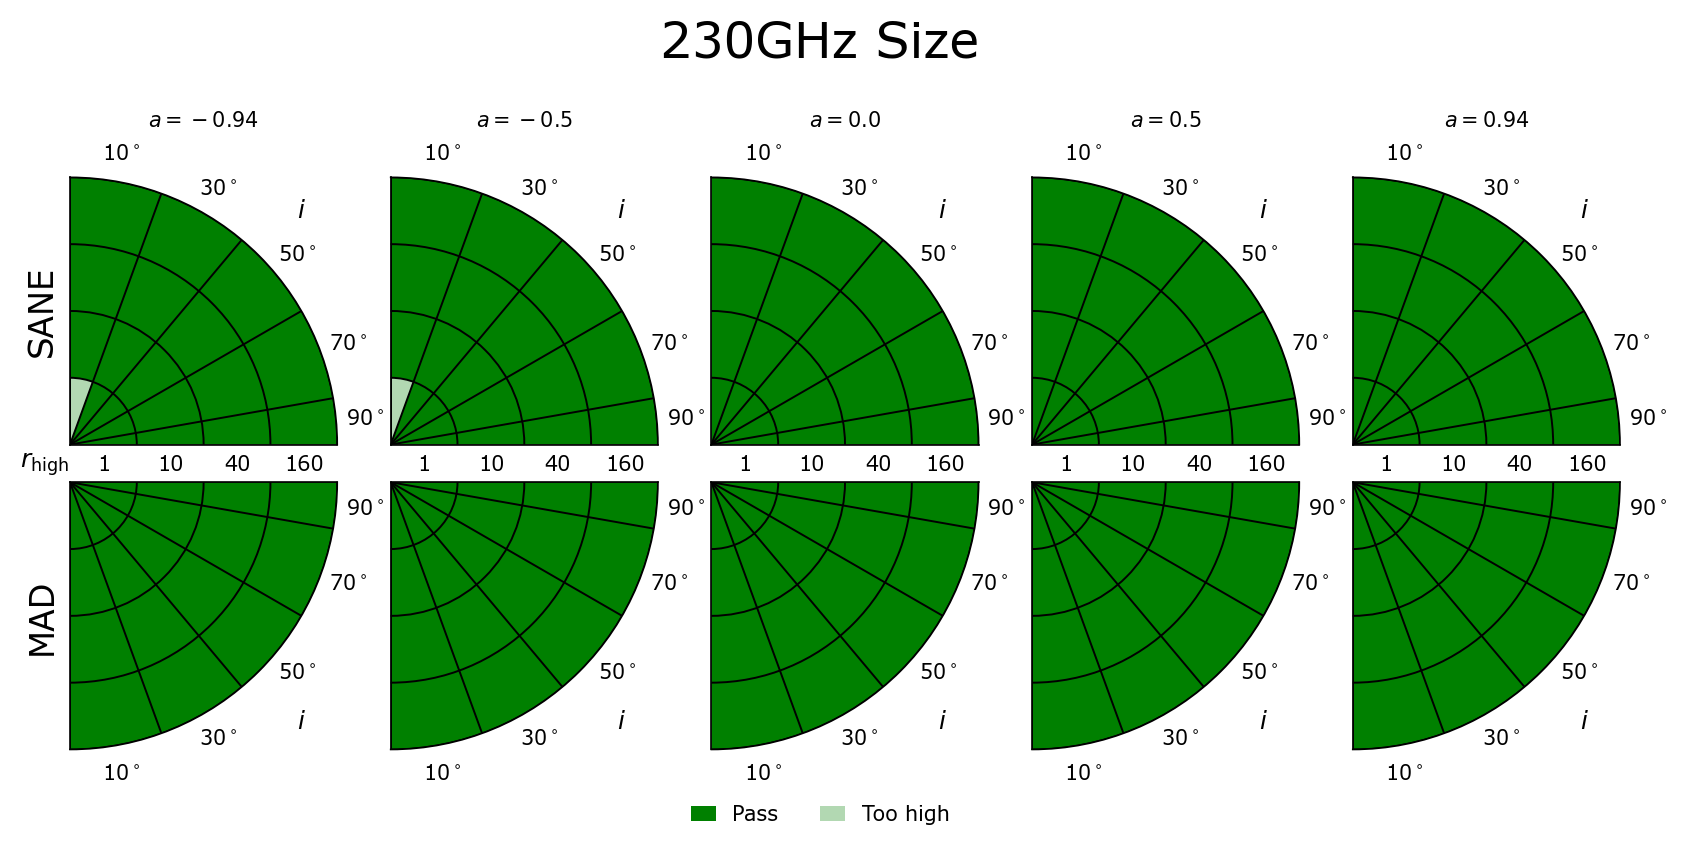
\includegraphics[width=\columnwidth]{./figures/230GHz_size_Constraints.png}
%  \caption{2nd moment plots}
%  \label{fig:cmp_2nd_moment}
%\end{figure}

The second moment constraint rejects only 1.5\% of models: nearly all models are about the right size.  The rejected models are $\abh \le 0$, face-on, SANE models with $\Rh = 1$.  These models have extended emission that is large compared to the critical impact parameter $b_c = \sqrt{27} \rg$.  The right panel of Figure~\ref{fig:passfail_sz} shows one of these failed models.

%..............................................................................
\subsubsubsection{Visibility Amplitude Morphology}

% Statement about consistency between overlapping model sets.

\begin{figure*}
  \centering
  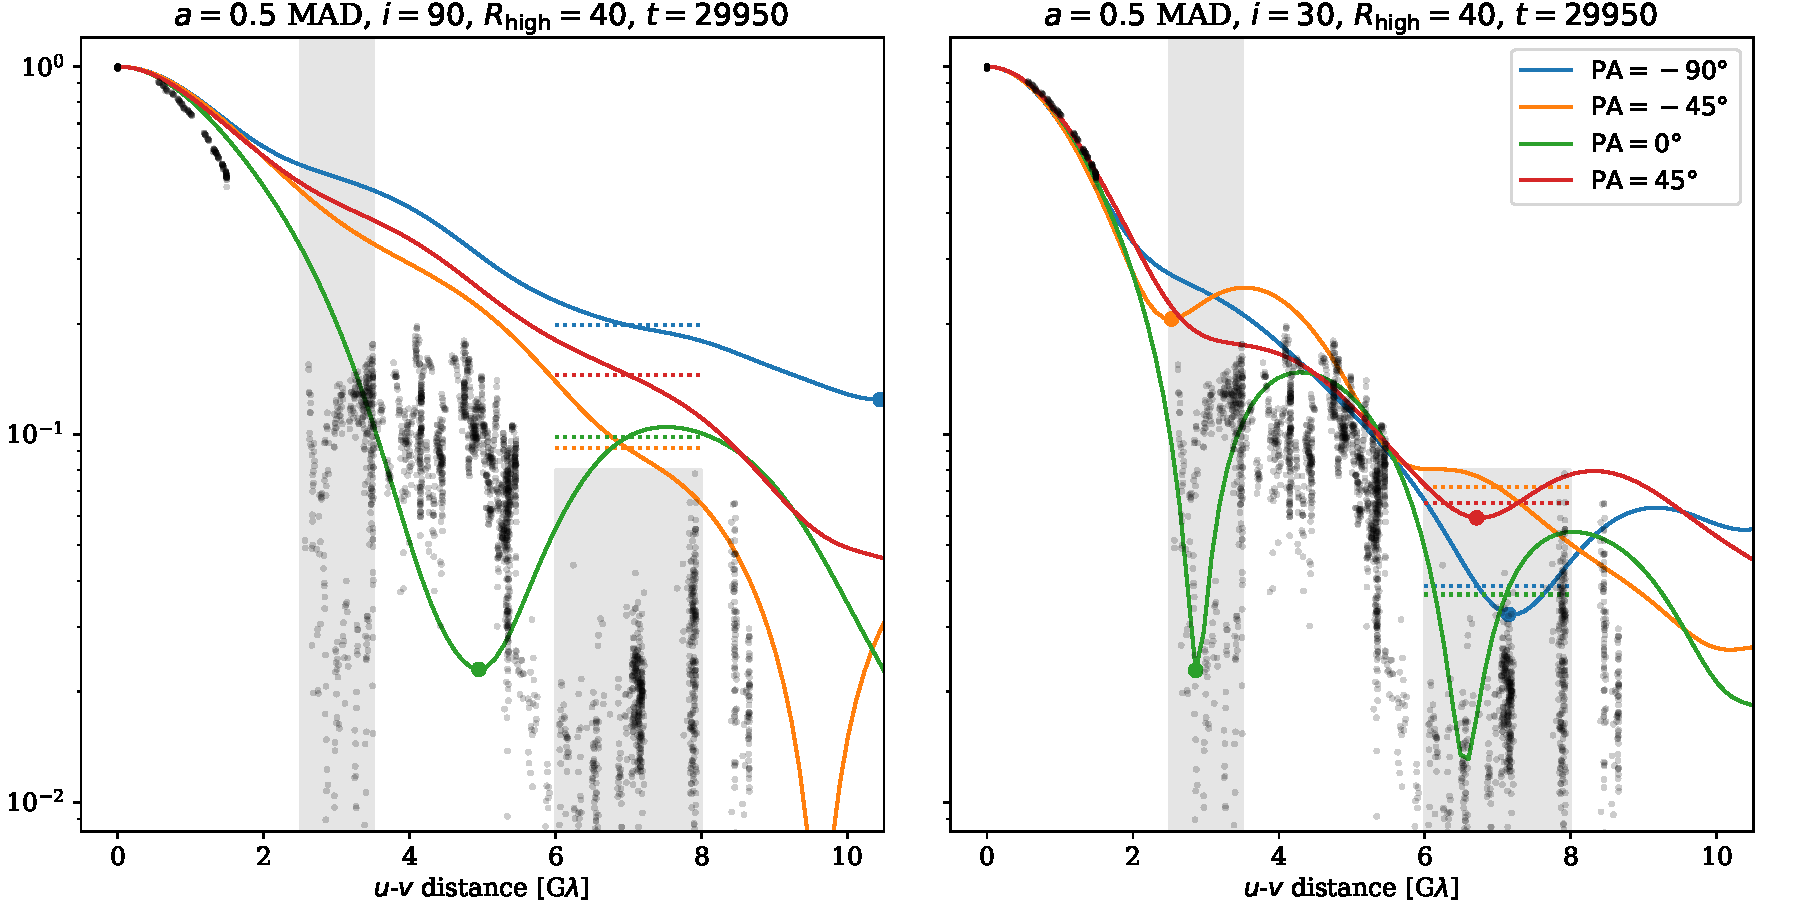
\includegraphics[width=0.75\textwidth]{figures/passfail_va.pdf}
  \caption{Visual representation on how the \vam constraint work.
    For each of the panels, we select a snapshot from a model and plot
    its visibility amplitudes as functions of the $(u,v)$ distance at
    position angles $-90\degree$ (horizontal), $-45\degree$,
    $0\degree$ (vertical), and $45\degree$.
    Because of the Hermitian symmetry, they cover 8 position angles in
    the image domain.
    The EHT \aprilvii VLBI data points are plotted as black circles.
    Even without further details, it is clear that the model on the
    left matches reasonably well with the data; while the model on
    the right is completely off.
    The \vam constraint is designed exactly to rule out models like
    the one on the right.
    As a visual guideline, the vertical gray band between 2.5 and
    3.5$\,\mathrm{G}\lambda$ marks the allowed null location in the
    \vam constraint; and the gray region between 6 and
    8$\,\mathrm{G}\lambda$ marks both the $(u,v)$ distance range for
    computing the long-baseline median amplitude and its allowed
    values $\mathrm{median}[V(6\,\mathrm{G}\lambda \leq \lambda \leq
      8\,\mathrm{G}\lambda)] \leq (4\%/50\%) V_0$.
    We numerically find the first local visibility minima along each
    position angle and show them as solid points.
    We also compute the median visibility amplitude in the marked
    region along each position angle, which are marked by dotted lines.
    A model is rejected if \emph{all} the first nulls land
    \emph{outside} the virtual gray band, or if \emph{any} of these
    lines land \emph{outside} the horizontal gray band.
    For the examples in this figure, the left model passes the \vam
    constraint because one of the first null (green dot) falls within
    the allowed range; and none of the long-baseline median (all
    dotted lines) go above 4\%/50\%.
    The right model fails the \vam constraint because both of the null
    location and long-baseline VAs are off.}
  \label{fig:passfail_va}
\end{figure*}

\begin{figure*}
  \centering
  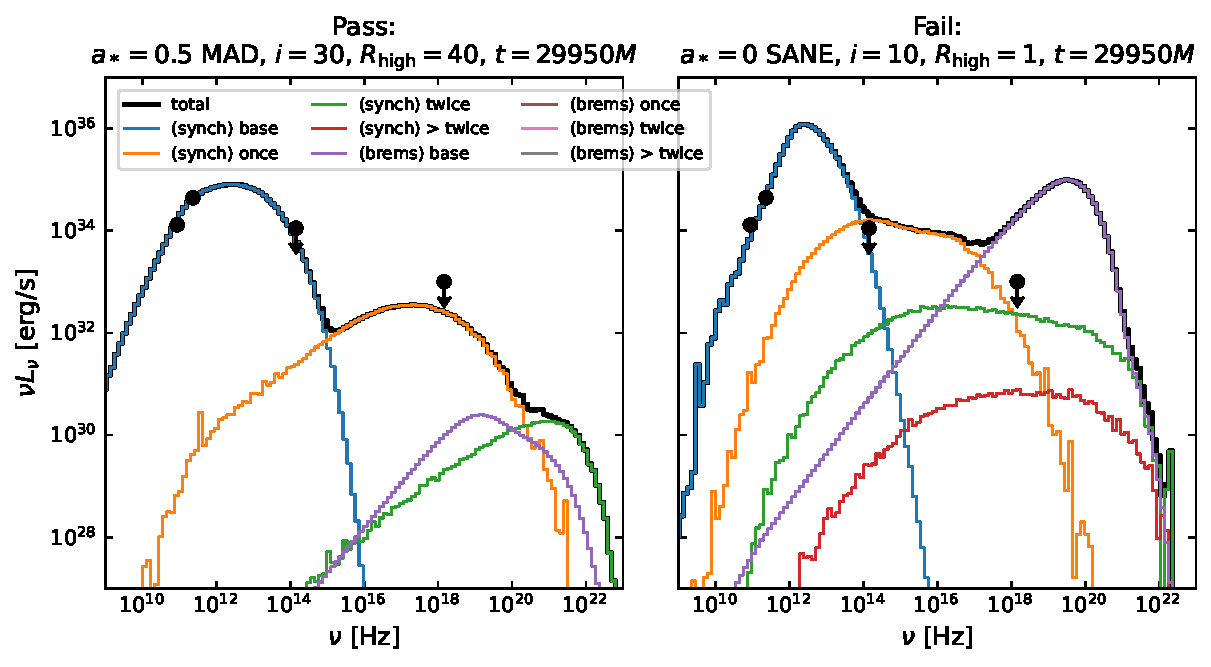
\includegraphics[width=0.75\textwidth]{figures/passfail_sed.pdf}
  \caption{\ckc{We may skip this figure given
      Fig.~\ref{fig:sample_seds} is similar.}
    Visual representation on how the non-EHT flux constraints work.
    This figure is similar to Figure~\ref{fig:sample_seds} but, in
    addition to show a model that works (left panel), we purposely
    select a model that fails both both the NIR and x-ray constraints.
    The right panel is a zero-spin face-on SANE with $\Rh = 1$.
    Because of high electron temperature, the synchrotron at $\sim
    10^{12}\,\mathrm{Hz}$ peak at $\sim 10^{36}\ergsps$, which creates
    a significant inverse Compton component that pushes the NIR beyond
    the limit.
    For the x-ray ray, this model follows the typical SANE behave and
    overproduce thermal Bremsstrahlung.}
  \label{fig:passfail_sed}
\end{figure*}

%\begin{figure}
%  \centering
%  \includegraphics[width=0.5\textwidth]{figures/va_compare.pdf}
%  \caption{Visibility amplitude as a function of baseline length
%    observed on 2017 April 7.
%    The pink band marks the location of the first minima in the
%    visibility amplitude along different orientations.
%    The horizontal red line marks our conservative upper limit for the
%    observed visibility amplitude between $6-8$G$\lambda$.}
%  \label{fig:cmp_null}
%\end{figure}

%\begin{figure}
%  \centering
%  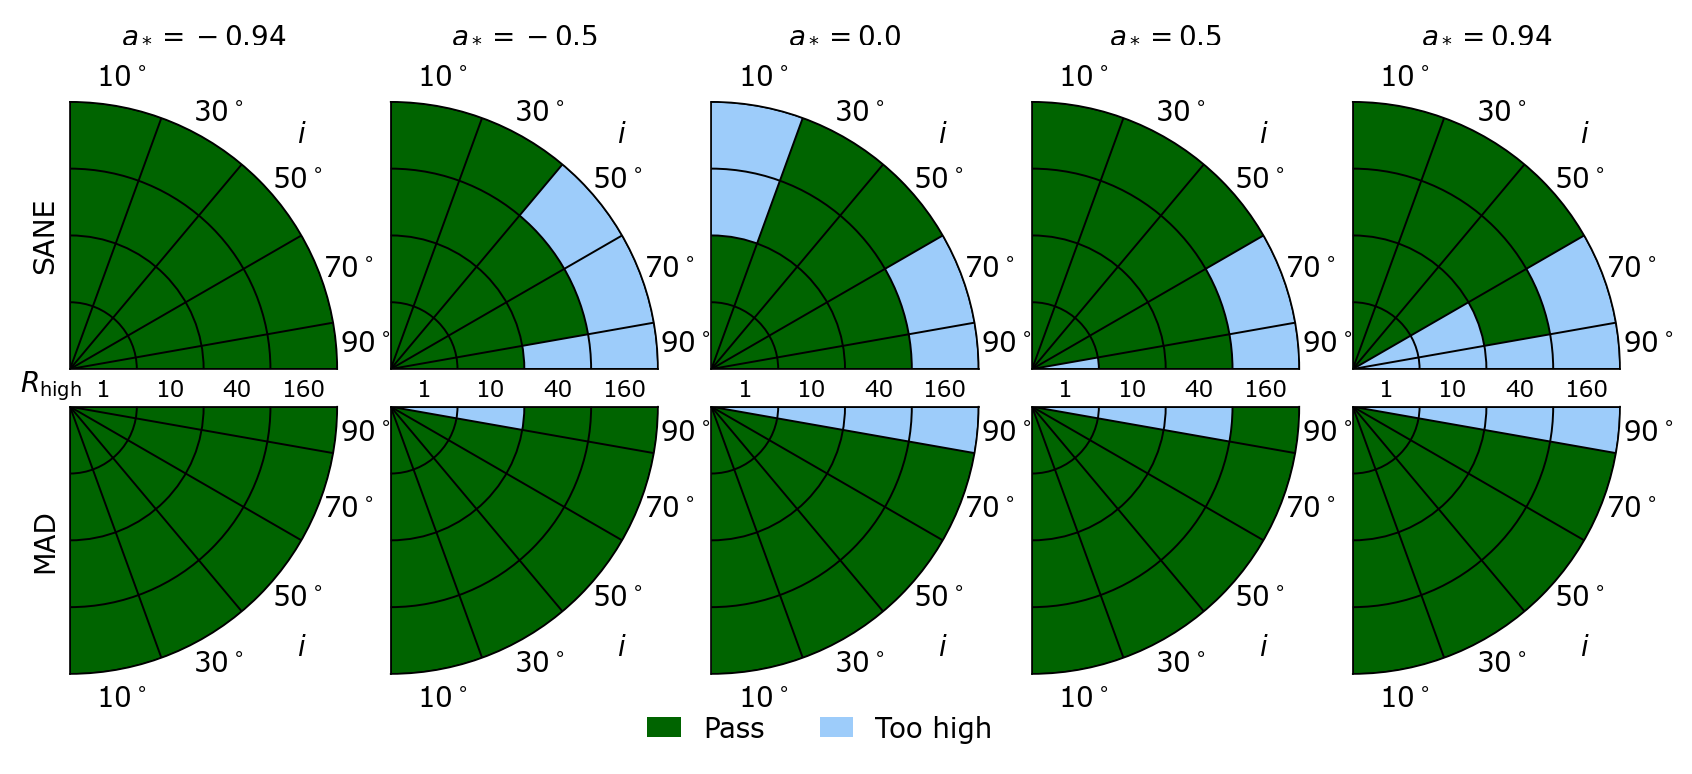
\includegraphics[width=\columnwidth]{./figures/Null_loc_Constraints.png}
%  \caption{Null Location Constraint\ckc{Texts/labels in pizza plots too %small to read.}}
%  \label{fig:cmp_ozel}
%\end{figure}

The \vam constraint checks if the VAs of a model roughly matches the
observation by comparing its null location and long-baseline visibility
amplitude.
As Figure~\ref{fig:passfail_va} demonstrates, this constraint is
informative.
It matches the ring size by using the null location, and the ring
width by using the long-baseline amplitude.
The test rejects edge-on MAD models at positive spin and a few large
$\Rh$ SANE models.
It disfavors edge-on MAD models at positive spin and a few large $\Rh$
SANE models.
The null location constraint rejects 16\% of models in total.

%..............................................................................
\subsubsubsection{M-ring Fits}
\label{sec:mring}

The m-ring fits reject 7\%, 33\%, and 65\% of models for the ring asymmetry, diameter, and width respectively.

The asymmetry parameter is typically not well constrained. Most rejected models are high inclination MAD models with $\abh \ge 0$.  Most of the rejected models have asymmetries that are large and detectable because Doppler boosting concentrates emission in an equatorial spot on the approaching side of the disk.

%\begin{figure*}
%  \centering
 % 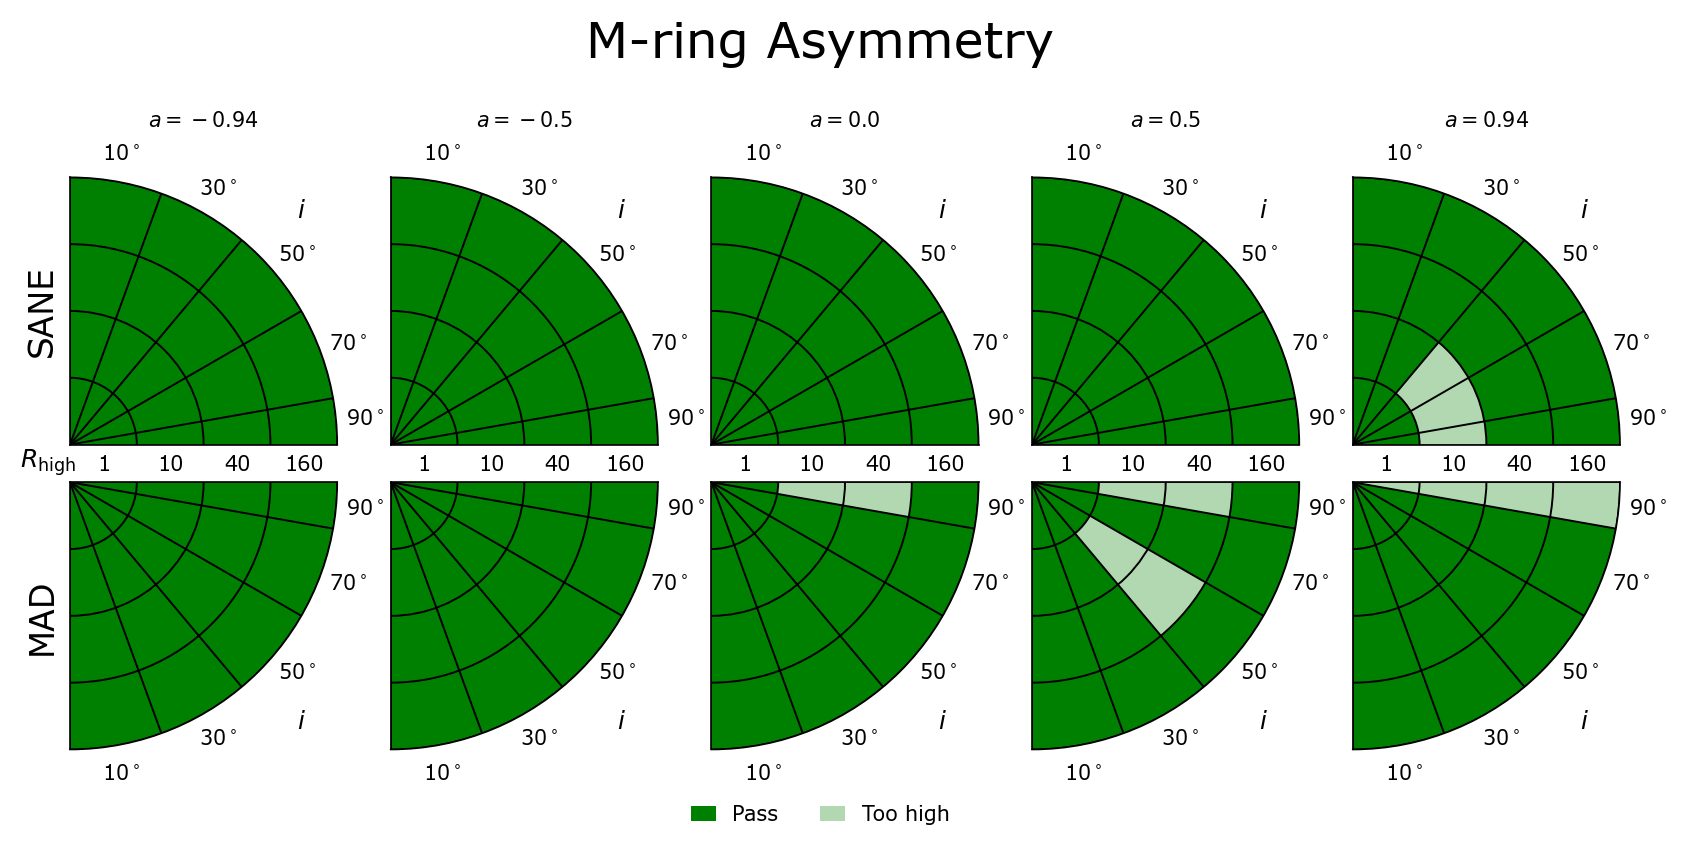
\includegraphics[width=\columnwidth]{./figures/Mring_f1_Constraints.png}
%  \caption{m-ring asymmetry}
%  \label{fig:cmp_m-ring_asymm}
%\end{figure*}

The ring diameter is better constrained than the asymmetry parameter.  It also varies systematically from model to model.  For example, the distribution of diameters is much broader at $\Rh = 1$ than at larger values of $\Rh$.  More models therefore fail the ring diameter test.

Most of the models that fail are low inclination models with ring diameters that are too large (no models fail because the ring diameter is too small).  For example, the face-on, $\Rh = 10$ SANE models fail for all spins except $\abh = 0.94$ because the ring is too large.  The same is true for all face-on MAD models with $\Rh = 1$.

Notice that the ring diameter is not degenerate with the second moment constraint; all models that fail the latter pass the former.  Recall that in addition to a blurred ring, the m-rings model contains a centered Gaussian component; the Gaussian tends to grow to absorb the emission when the ring is very extended.

The distribution of ring diameters for many SANE models is multimodal (consistently in the Frankfurt and Illinois \monika{can we stop calling these models Illinois or Frankfurt models???} model sets), with a secondary peak in the distribution at $\sim 35\mu$as.  All $\Rh = 1$ SANE models show this secondary peak.  These models' images tend to have a well defined ring at the critical impact parameter and a second broad maximum in intensity at larger impact parameter.  The second peak in the distribution is a consequence of limited baseline coverage.

%\begin{figure*}
%  \centering
%  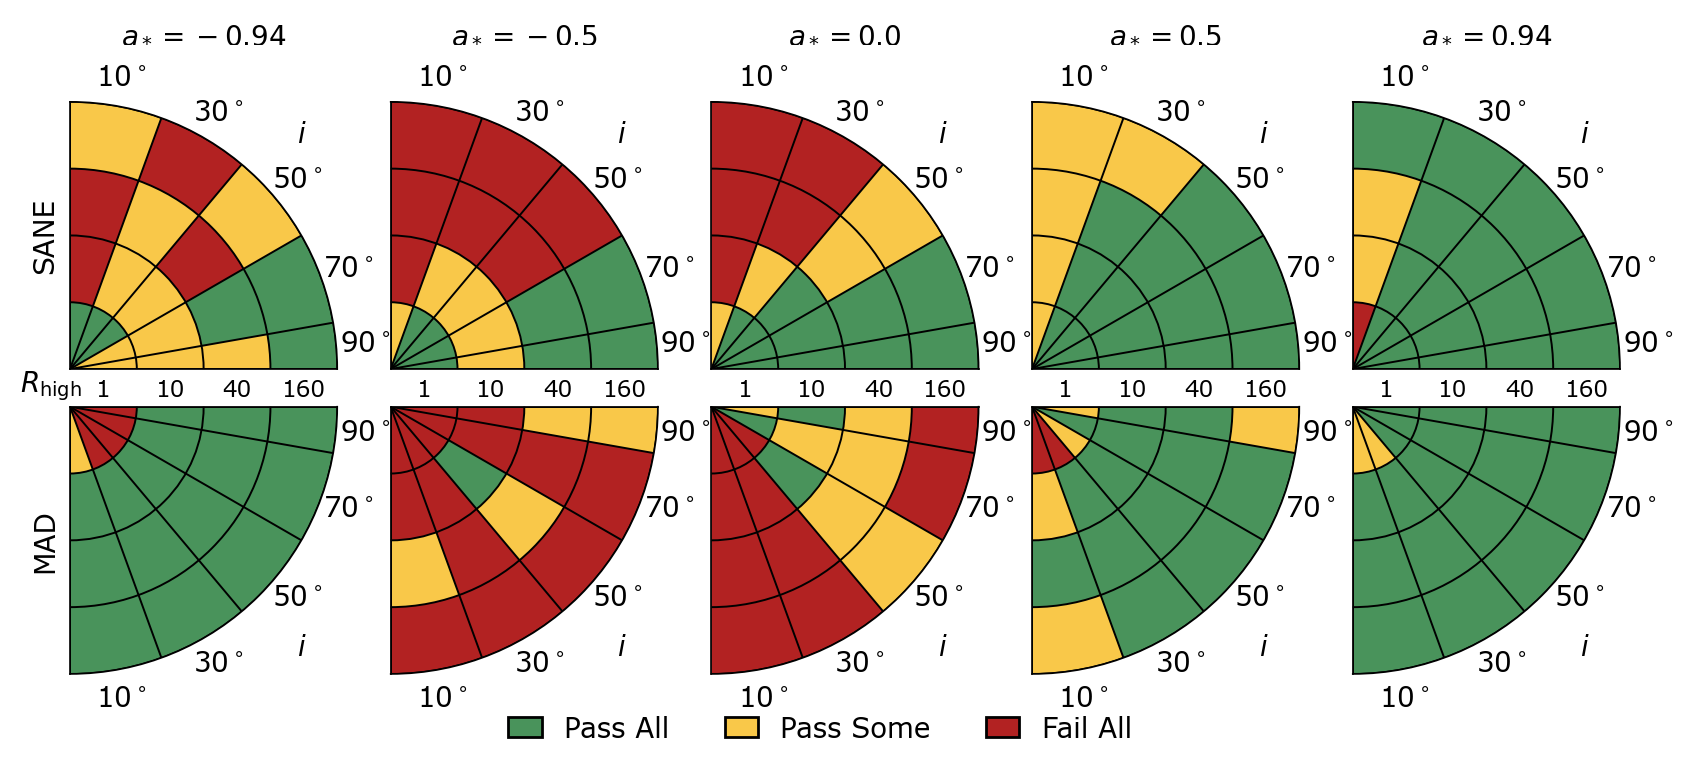
\includegraphics[width=\textwidth]{./figures/Mring_d_Constraints.png}
%  \caption{M-Ring diameter.}
%  \label{fig:cmp_m-ring_diam}
%\end{figure*}

The m-ring width $w$ is the most tightly constrained of our 3 parameters.  Although the closure phases constrain $w$ as well, it is easy to see how $w$ affects visibility amplitudes at long baselines.  For example, for a simple, symmetric ring the visibility amplitudes are a Bessel function multiplied by a Gaussian with width $\sim 1/w$, and increasing $w$ therefore decreases the amplitude of the long baselines.

All rejected models have median $w$ that is below the median of the data, $ \simeq 17.5\mu$as. The rejected models include all but 3 MAD models at $\abh \le 0$ and all edge-on ($i = 90\degree$) MAD models.  MAD models exhibit a strong trend toward smaller $w$ as $i$ increases.  SANE models exhibit a similar but weaker trend. The SANE model images have  higher optical depth, broader rings, and more substructure than the MAD models.  Their $w$ distributions are typically broad, with mode well below $17.5\mu$as.  Only for $\abh = 0.94$, where the optical depth is lowest due to higher temperatures in the emitting region, do most of the models exhibit a sharply peaked $w$ distribution centered at $17.5\mu$as.

\begin{figure*}
 \centering
 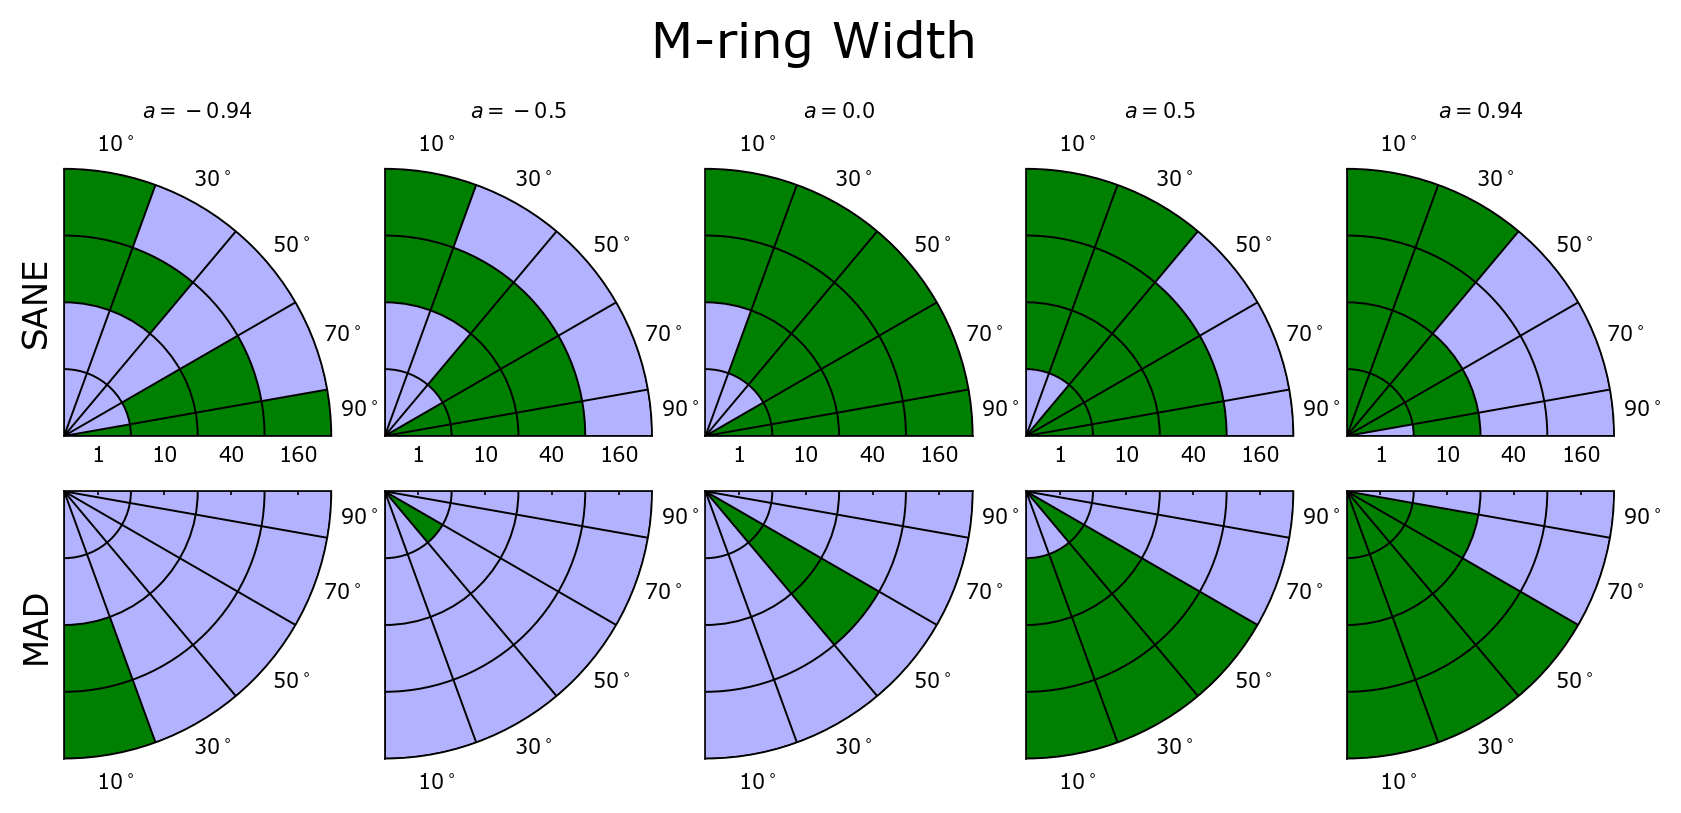
\includegraphics[width=\textwidth]{./figures/Mring_w_Constraints.png}
  \caption{Pass/fail plot for the m-ring widths.}
% \label{fig:cmp_m-ring_width}
\end{figure*}

%..............................................................................
\subsubsubsection{EHT Constraint Summary}

We can combine all EHT constraint cuts with a logical {\em and} operation.  The results are summarized in Figure~\ref{fig:all_EHT_constraints}.  Evidently EHT data alone is capable of discriminating between models.   The edge-on ($i = 90\degree$) MAD models all fail, with some failing m-ring width, diameter, asymmetry and the null location constraint.  The cuts clearly favor $\abh > 0$ models, although there are exceptions.  We are left with $33/100$ SANE models and $16/100$ MAD models.

\begin{figure*}
  \centering
    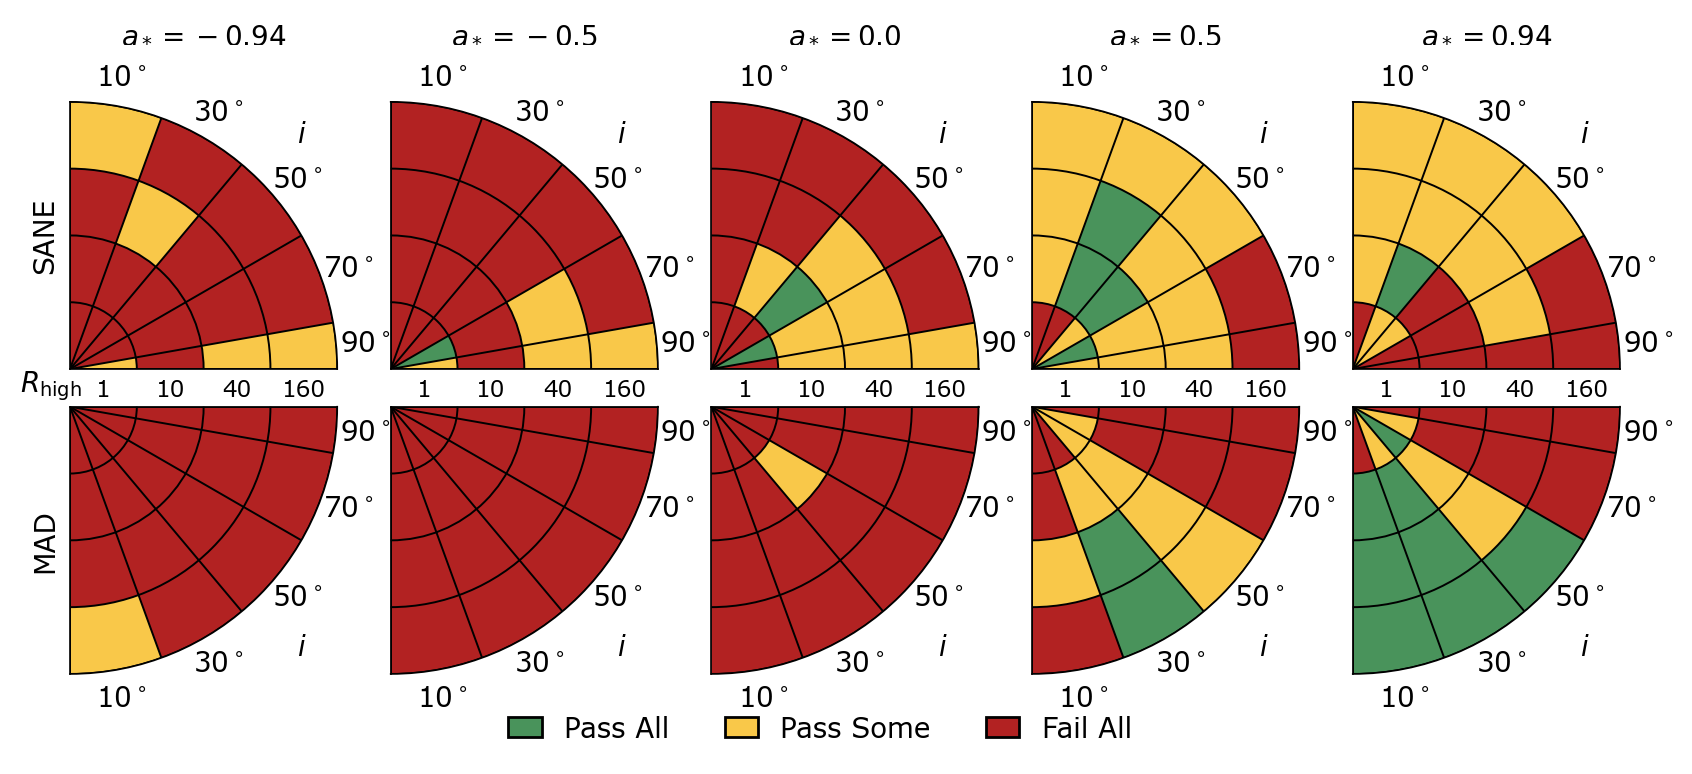
\includegraphics[width=\textwidth]{./figures/Interferometric_Constraints.png}
  \caption{Combined EHT constraints (logical {\em and}) including the second moment, null location, and m-ring fit constraints.}
  \label{fig:all_EHT_constraints}
\end{figure*}

%------------------------------------------------------------------------------
\subsubsection{Non-EHT Constraints}

Now consider constraints from unresolved 86\GHz, NIR, and X-ray
observations.
Some or all of the emission in these bands are believed to originate
in the compact source from plasma that is close to or overlaps the
plasma that is producing the 230\GHz-emitting plasma observed by EHT.
While we will go through each of the constraints one-by-one,
Figure~\ref{fig:passfail_sed} compares models that pass and fail these
constraints.

%..............................................................................
\subsubsubsection{NIR Median Flux}

NIR photons are produced by the synchrotron process from electrons on the high energy end of the eDF.  For the one-zone model with $B = 30$G and $\Theta_e = 10$ the mean Lorentz factor is $\gamma = 30$ and the synchrotron critical frequency $\nu_{crit} = \gamma^2 e B/(2 \pi m_e c) \simeq 80\GHz$.  Emission at $2.2\um$ is therefore produced by electrons with  Lorentz factor $\gamma \simeq 10^3$.  NIR flux density will therefore be sensitive to $\Theta_e$ and $B$.  Since both increase toward the horizon, and field strength is nearly independent of latitude, NIR photons are produced at small radius in regions where $\Theta_e$ is highest.

The sensitivity to $\Theta_e$ implies that NIR will be strongest for parameters with higher temperatures.  For SANEs the midplane temperature increases with $\abh$.
The sensitivity to $B$ implies that NIR will be strongest for parameters with stronger fields.  The $B$ depends on the GRMHD flow configuration and also on the mass unit (that is, the accretion rate), and so NIR will be strongest when the accretion rate is largest.  For SANEs, accretion rate declines as $\abh$ increases and $\Rh$ decreases (see Figure \ref{fig:accretion_outflow_power_illinois_thermal} below); for MADs the accretion rate dependence on $\abh$ and $\Rh$ is much weaker.
Finally, Doppler effect (blueshift) enables photons that are detected at $2.2\mu$m to be emitted at longer wavelength in plasma that is moving toward the observer, and the accompanying Doppler beaming increases the detected intensity.  We therefore expect that NIR to increase with inclination and to peak in the midplane on the approaching side of the flow.

Models that pass the NIR flux limit are shown in the Appendix in Figure~\ref{fig:2um_flux_pizza}. The rejected SANE models ($6\%$) tend to be at positive spin and high inclination, and the images are dominated by a bright spot on the approaching side of the disk.
The rejected SANE models ($68\%$) include all models at $\Rh = 1$ and all but 2 models at $\Rh = 10$, where $\Theta_e$ tends to be larger, and {\em all} edge-on models, where Doppler boosting is largest.

Interestingly, we find that some models are Compton dominated in the NIR.  For example, $\abh = -0.94$ SANE models become optically thin at relatively low frequency as $\Rh$ goes to $1$, and thus synchrotron emission drops off rapidly as frequency increases.
As $\Rh$ drops and synchrotron decreases the SED becomes dominated by a lower-luminosity bump of underlying Comptonized photons.  Just before this happens, at $\Rh = 10$, the combination of the Compton bump and synchrotron emission is enough to push the median NIR flux density above the observational limit, explaining the excluded SANE models at $\Rh = 10$, $\abh = -0.94$.

%\begin{figure}
%  \centering
%  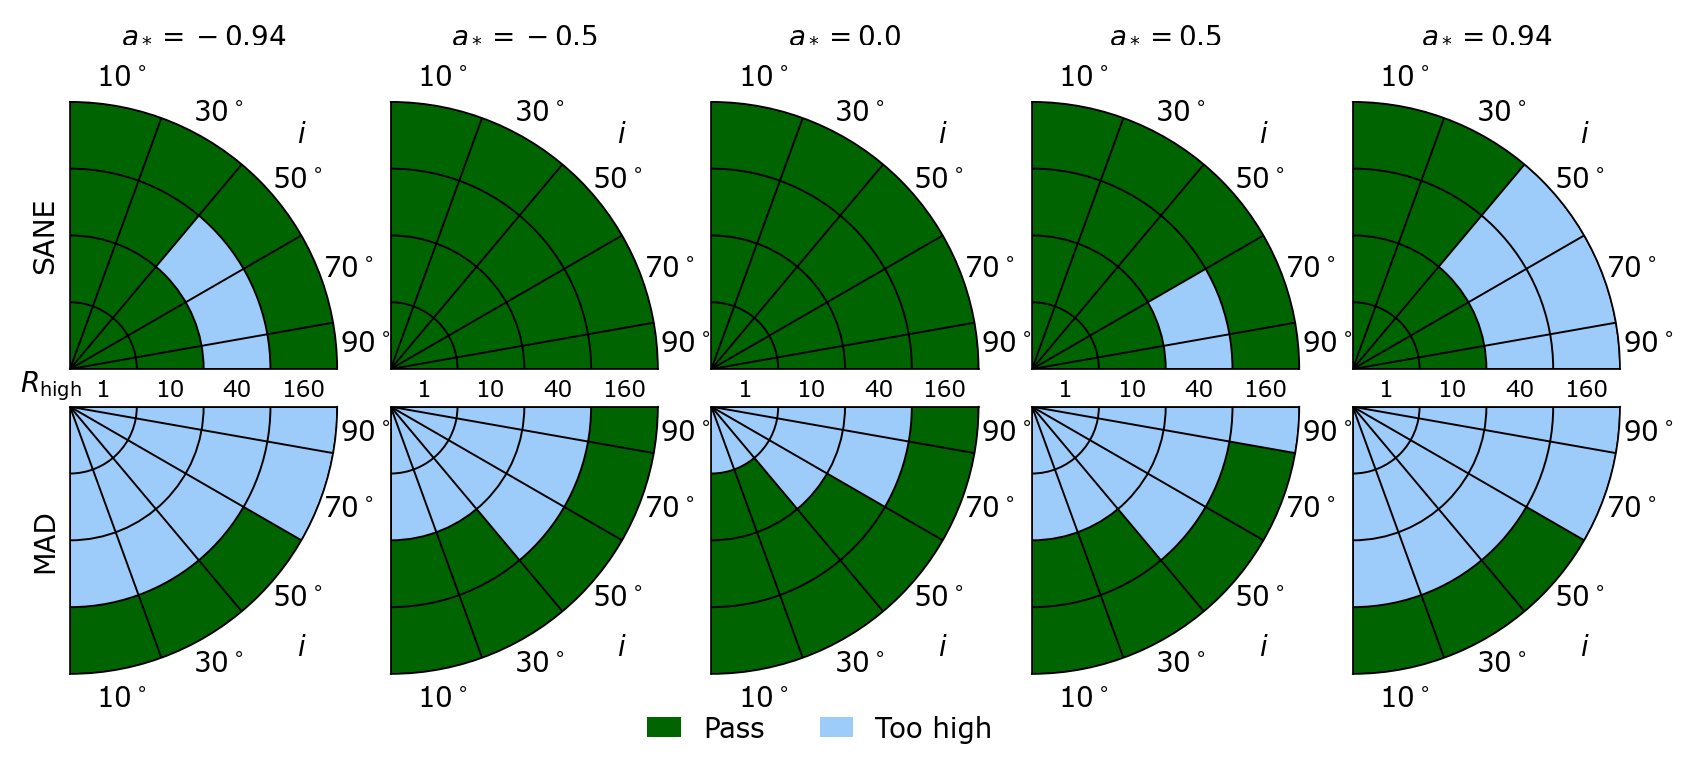
\includegraphics[width=\columnwidth]{./figures/2um_flux_Constraints.png}
%  \caption{NIR flux limit}
%  \label{fig:cmp_2um_flux}
%\end{figure}

%..............................................................................
\subsubsubsection{X-ray Luminosity}

Many thermal models produce X-ray emission through Compton upscattering of thermal synchrotron photons.  In the first Compton bump $\nu L_\nu$ is proportional to the y-parameter $y \sim 16 \Theta_e^2 \tau_e$ where $\tau_e$ is a characteristic electron-scattering optical depth and $\Theta_e$ is a typical electron temperature.  At $\Rh = 1$ the X-ray band lies in the first Compton bump, while at larger $\Rh$ the bumps move to lower energy because the bulk of the Thomson depth is in the midplane where $\Theta_e \propto 1/\Rh$.

In many large $\Rh$ SANE models, however, X-ray emission is dominated by bremsstrahlung.  Since its emissivity $j_{\nu,b} \propto n^2$, bremsstrahlung is dominated by regions with the highest density, i.e. the midplane.  It typically comes from larger radius than the synchrotron and Compton-upscattered X-ray emission and therefore varies more slowly.  Bremsstrahlung therefore dominates Compton in the highest accretion rate models, i.e. when $\Rh$ is large (see Section~\ref{sec:discussions}).  Notice that $j_{\nu,b} \propto \Theta_e^{1/2}$ for $\Theta_e > 1$ and $\Theta_e^{-1/2}$ for $\Theta_e < 1$, so cool disks enhance bremsstrahlung.

The X-ray cut results are shown in Appendix~\ref{app:tables} in Figure~\ref{fig:xray_pizza}.

Most large $\Rh$ SANE models fail the X-ray test: all but 2/25 at $\Rh = 160$ and all but 2/25 at $\Rh = 40$.  These models fail due to excess bremsstrahlung.

The MAD models that fail have low $\Rh$ and are Compton-dominated in the X-ray.  All $\Rh = 1$ MAD models fail the X-ray test, and all but 6/25 at $\Rh = 10$.  The midplane $\Theta_e$ declines as $\Rh$ drops.  Since the midplane contributes most of the electron scattering optical depth, low $\Rh$ models have the largest $y$ parameter and are at greatest risk of overproducing X-rays.

%\begin{figure}
%  \centering
%  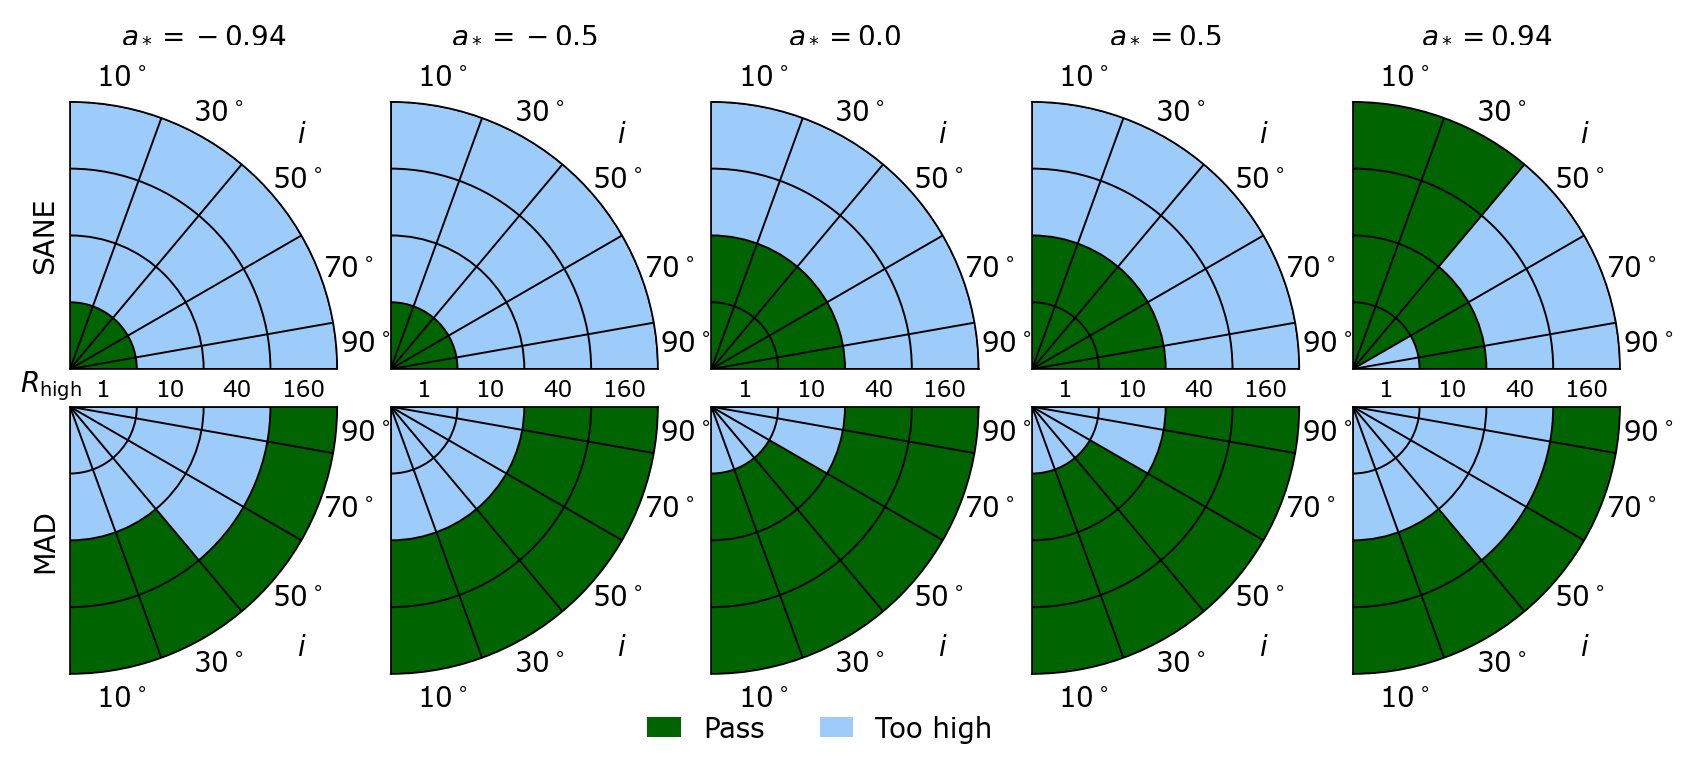
\includegraphics[width=\columnwidth]{./figures/Xray_flux_Constraints.png}
%  \caption{X-ray flux limits}
%  \label{fig:cmp_xray_flux}
%\end{figure}

%..............................................................................
\subsubsubsection{86\GHz Median Flux}

In a naive picture \sgra's millimeter flux is produced in a photosphere that decreases in size as frequency increases.  Because optical depth is not large at $1.3$mm ($\sim 0.3$ in the one-zone model) and the source structure is complicated (the optical depth varies across the image; the $\tau = 2/3$ surface is non-spherical, folded, and not even simply connected) the naive picture is imprecise.  Nevertheless 86\GHz photons are on average produced at larger radius than 230\GHz photons, and the 86\GHz source size is larger than the 230\GHz source size.

The 86\GHz/230\GHz color is therefore sensitive to the radial structure of the source plasma.  Figure \ref{fig:86GHz_flux_pizza} shows the full results of applying this constraint.

\cfg{need more physical discussion}

Many $\Rh = 1$ models, both MAD and SANE, fail the 86\GHz flux density test: 22/25 SANE and 11/25 MAD; all overproduce 86\GHz emission.  A large set of SANE models (17/100) underproduce 86\GHz emission, and these have $10 \le \Rh \le 40$.

The 86\GHz flux is sensitive to $\Rh$.  For example, SANE $\abh = 0$, $i = 70,90$deg models are too bright at $\Rh = 1$ and too dim at $\Rh = 10$.  There must be passing models in between, suggesting our parameter space is not sampled densely enough.

%\begin{figure}
%  \centering
%  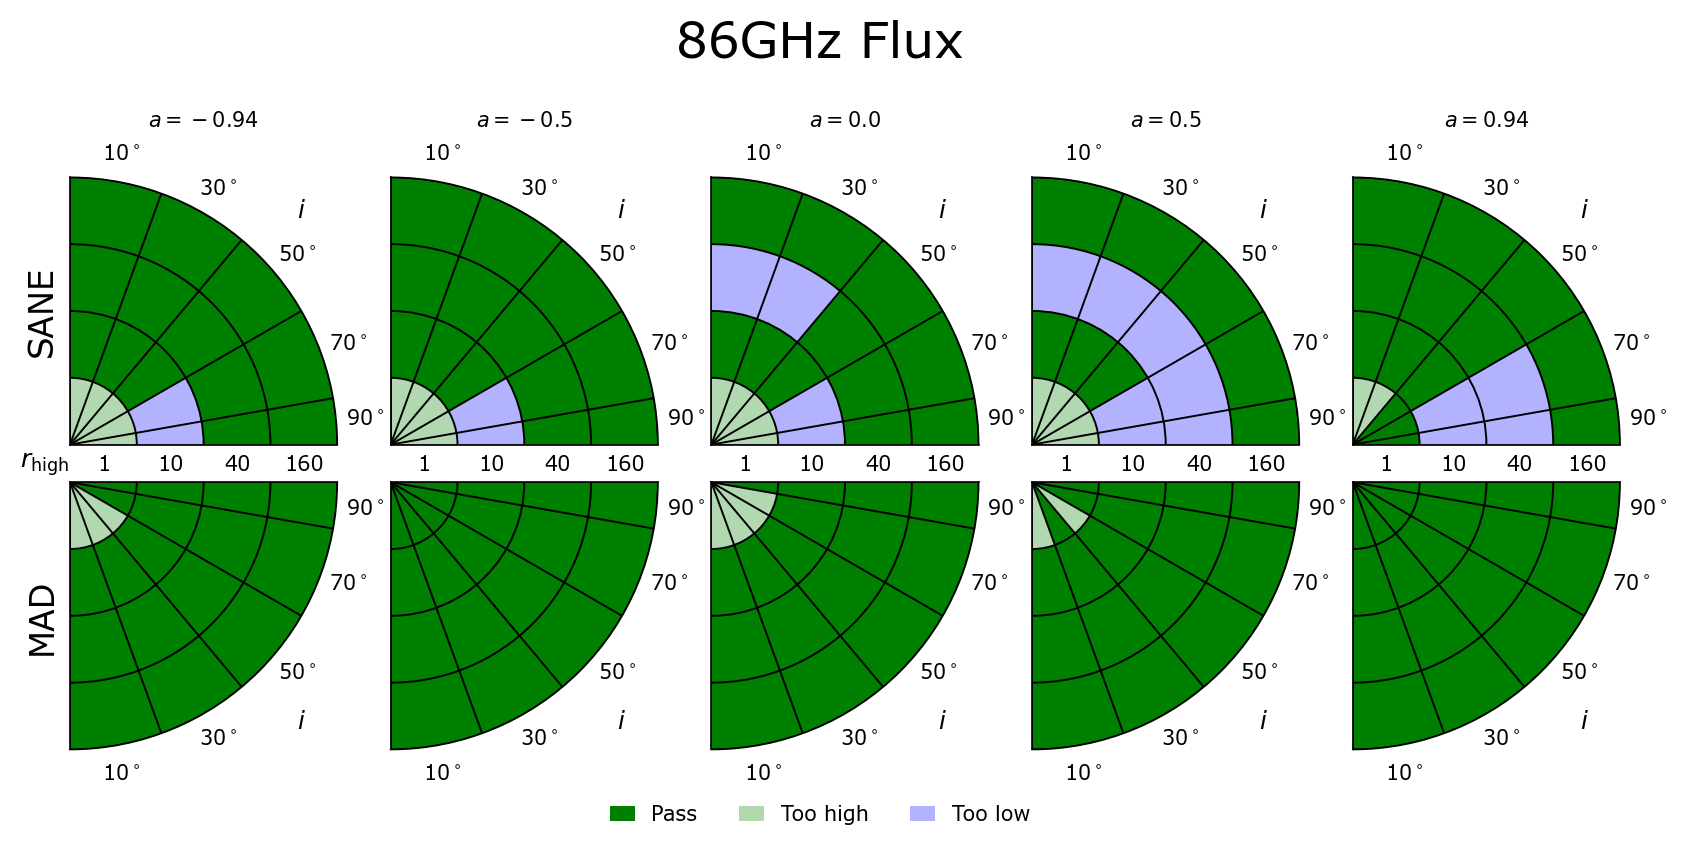
\includegraphics[width=\columnwidth]{./figures/86GHz_flux_Constraints.png}
%  \caption{86GHz flux limits}
%  \label{fig:cmp_86ghz_flux}
%\end{figure}

%..............................................................................
\subsubsubsection{86\GHz Major Axis}

As for the 86\GHz flux, the 86\GHz size is sensitive to optical depth as a function of radius in the source plasma. Figure~\ref{fig:86GHz_size_pizza} in Appendix~\ref{app:tables} shows the full results of applying this constraint.

\cfg{need cites to earlier work for par below}

The 86\GHz size is sensitive to inclination.  For example, the MAD, $\abh = 0$, $\Rh = 160$ models are too small at low inclination and too large when seen edge-on, because the edge-on models have prominent limb-brightened jet walls that are visible to 100$\mu$as.  The 86\GHz size constraint rejects
$58\%$ of models and is therefore one of the tightest constraints.

The physical picture for 86\GHz source size is complicated, as is the extraction of the constraint itself from observations.  Notice that (1) two different values for the 86\GHz intrinsic source size have been reported in the literature; (2) scattering is $7$ times stronger at 86\GHz than at 230\GHz; (3) scattering must be subtracted accurately to obtain the intrinsic source size; (4) the error bars for the 86\GHz source size are narrow and this plays a key role in determining the strength of the constraint.

%\begin{figure}
%  \centering
%  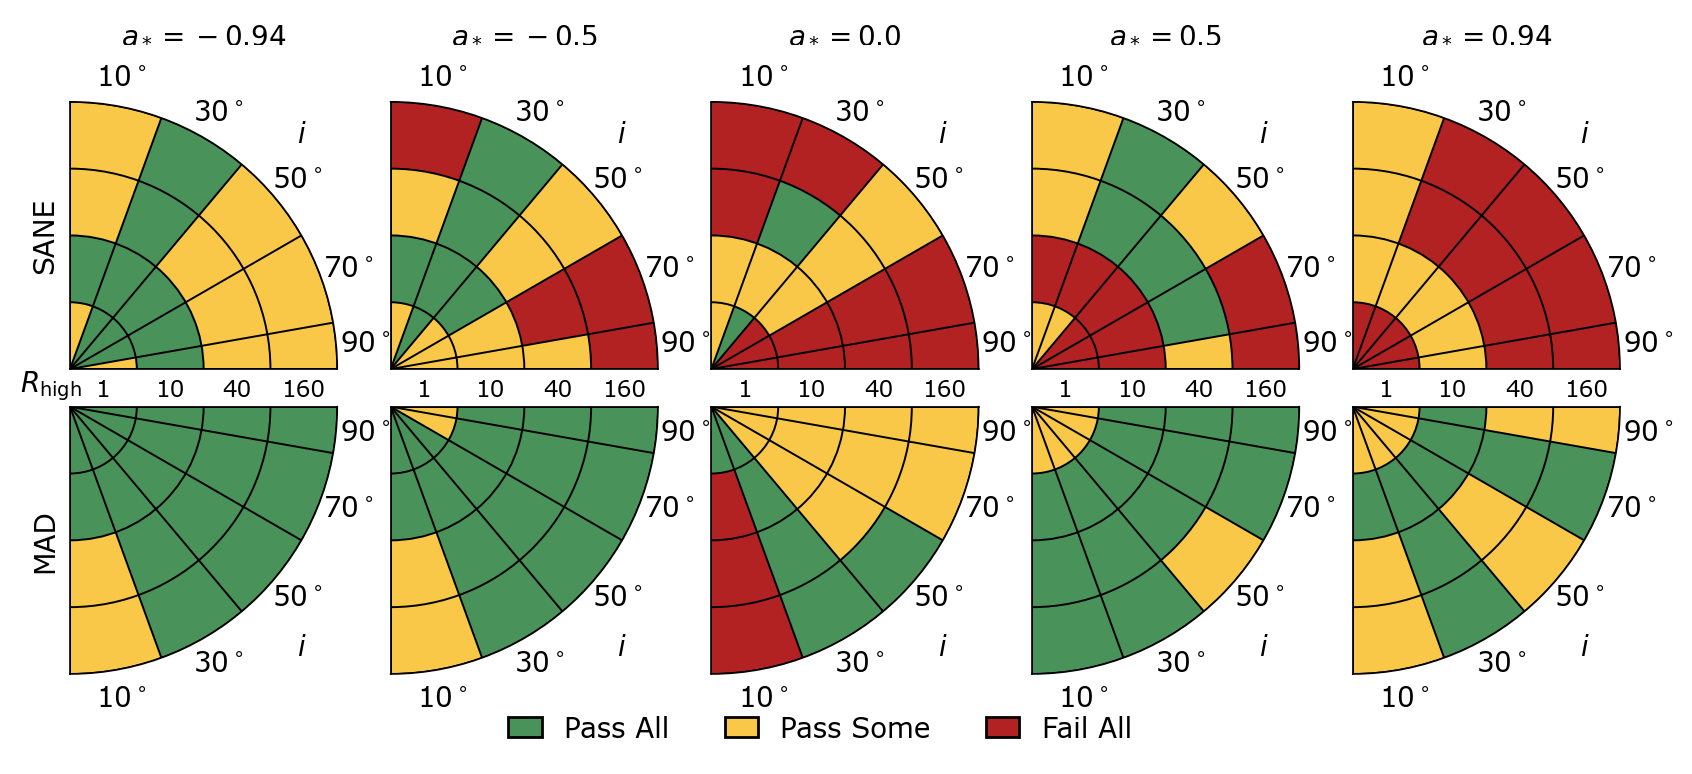
\includegraphics[width=\columnwidth]{./figures/86GHz_size_Constraints.png}
%  \caption{86GHz size}
%  \label{fig:cmp_86ghz_size}
%\end{figure}

%..............................................................................
\subsubsubsection{Summary of Non-EHT constraints}

Applying only non-EHT constraints, we are left with the 24/200 models shown in Figure~\ref{fig:non_eht_cuts}. The surviving models are the result of applying a heterogeneous and noisy set of constraints using a hard cutoff, which obscures the underlying physical pictures.  Nevertheless, the surviving models are nearly all MAD (only 1 SANE model survives), all have $\Rh > 1$, and nearly all are at $i \le 70\degree$.  This leaves a cluster of surviving MAD models at large $\Rh$ and moderate inclination.

\begin{figure*}
  \centering
  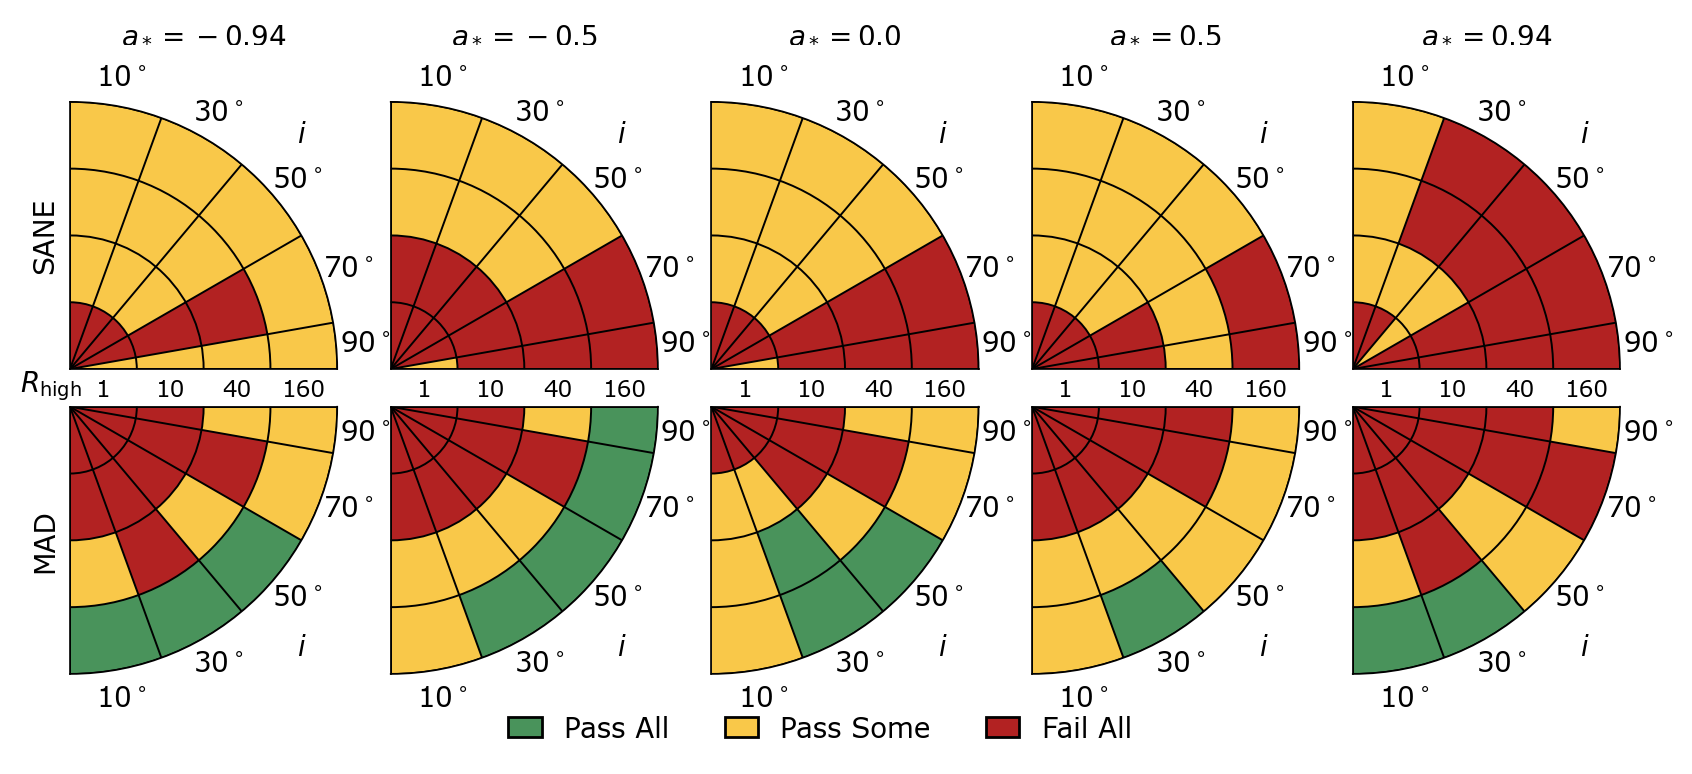
\includegraphics[width=\textwidth]{./figures/Non_Interferometric_Constraints.png}
  \caption{Combined non-EHT constraints}
  \label{fig:non_eht_cuts}
\end{figure*}

%------------------------------------------------------------------------------
\subsubsection{Variability}

Variability is central to interpretation of \sgra: an $8$hr observation of \sgra is $1400 \tg$, a timescale over which most models vary significantly.  In contract, an $8$hr observation of M87* is $\sim \tg$ and the source is hardly expected to vary at all.\footnote{This does not mean that \m87 is less variable than \sgra.  In 2017 EHT observed \m87 over only $\sim 19\tg$, so it is not possible to characterize \m87 variability using EHT data alone.  To obtain variability information for \m87 similar to what we present here for \sgra would require multi-year observations.}

Variability is a strong constraint.  Although models differ in their degree of variability, both in an integrated sense and on 4 $G\lambda$ baselines, only a small fraction of models are as quiet as the data.  For the light curve variability, this remains true whether we use data from 2017 April 7, all days from the 2017 observing campaign, or from historical monitoring of \sgra.   In general, we find that SANE models are quieter than MAD models, and (less strongly) face-on models are quieter than edge-on models.

If we were to apply the variability constraints directly to the models, there would be 37/200 successful models left using 1\% cuts (47/200 for the ALMA constraint and 121/200 for the visibility amplitude constraint).  One interpretation of this result is that the surviving models are the correct description of the source (although we would expect some misclassification of models as consistent or inconsistent when using 1\% cuts on such a large model set).  Another interpretation is that there is a missing physical ingredient in the models, and this possibility is discussed in Section \ref{sec:discussions}.

%..............................................................................
\subsubsubsection{ALMA Light Curve}

The distributions of 3 hour modulation index (rms \%) across all SANE models, across all MAD models, and across the historical dataset are shown in Figure \ref{fig:cmp_ALMA_var}, along with individual distributions for the models with the lowest and highest MI for SANEs and MADs. Although some individual models  pass (particularly SANE models), the distributions for the SANEs and the MADs are noticeably offset from the data, with the MADs in particular being more variable. As can be seen, even the quietest MAD model lies above the historical distribution.

If we compare each individual model to the three segments from the 7 April 2017 ALMA observation using a 2-sample KS test, eliminating models with $p < 1\%$, we are left with 56 SANE models and 9 MAD models.

If we instead compare the models to the full historical distribution (40 measurements of $\mi{3}$ in all, including ALMA), we find that 47 SANE models and no MAD models pass. This is more stringent than the comparison with just 7 April, since the historical distribution has more samples and thus disparate models can be eliminated with higher confidence.

\begin{figure}
  \centering
  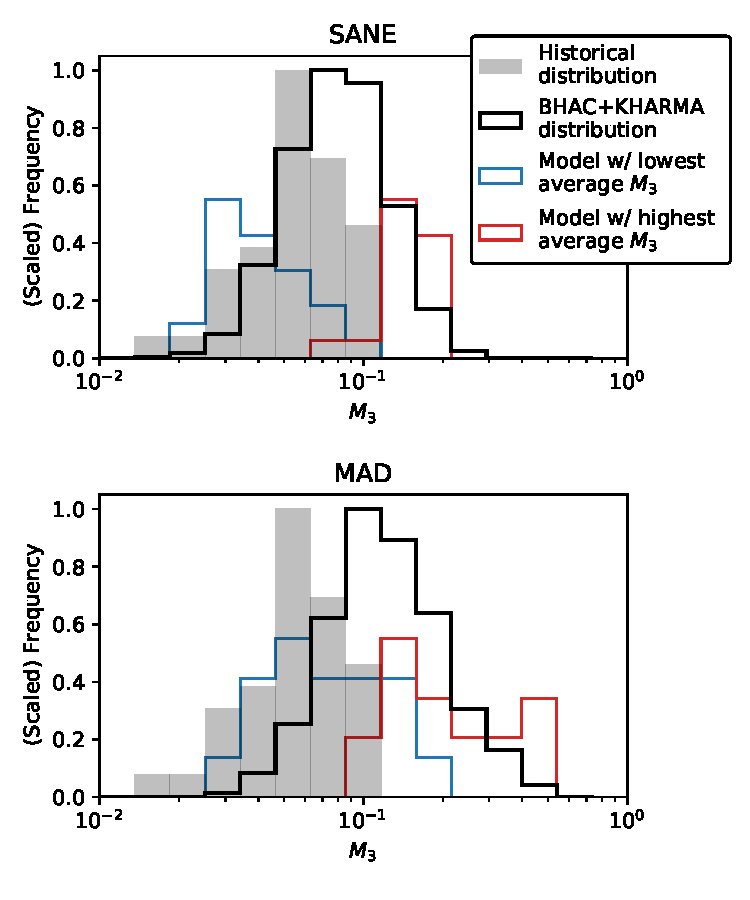
\includegraphics[width=\columnwidth]{./figures/mi_hist.pdf}
  \caption{Distributions of $\mi{3}$ for \kharma models (black), compared to distributions from historical observations (gray). The distributions for models with the lowest (blue) and highest (red) average $\mi{3}$ for SANEs and MADs are also shown. The heights of these distributions have been scaled down for visual clarity.
  }
  \label{fig:cmp_ALMA_var}
\end{figure}

%..............................................................................
\subsubsubsection{4 $G\lambda$ Visibility Amplitude Variability}

The power-law indexes of the variance $\sigma_\text{var}^2 (|u|)$ at $4~{\rm G}\lambda$ of the GRMHD models is generally in good agreement with the measured value of $b$ from the 2017 EHT campaign (excluding April 11). The amplitude $\afour^2$, however, varies depending on the model and the code.

Figure~\ref{fig:cmp_VLBI_var} shows the distribution of $(\afour^2, b)$ from the EHT observation, along with the distribution across all \kharma models. The GRMHD models are shown as an aggregate whole, but each model consists of only three measurements of $\afour^2$, one on each window. This makes a direct comparison with the measured value difficult, as the distribution for a given model is poorly constrained.

\citet{Georgiev_2022} gives an estimate for the width of the distribution as $\log_{10}(\afour^2) \pm 0.1$. We can get a rough estimate for how the GRMHD models fare compared to the measurement by taking the mean across windows and the estimate for the width, and comparing this with the measurement distribution under the assumption that both are distributed normally. Under this, 121/200 models (63 SANE and 58 MAD) agree with the data within 1\%, although we caution against interpreting this number as the number of passing or failing models, since the uncertainties in the model distribution are so large.

Overall, the GRMHD models tend to be slightly more variable than the measured value, with face-on models performing better than edge-on models. For SANE models, $\Rh = 10$ tend to be more variable than others. For MAD models, there is a slight preference for lower $\Rh$.

We have also considered a set of thermal, $\Rh$, MAD models run with the \koral code out to $\sim 100,000\tg$.  These models permit us to assess the importance of integration time for application of the constraints.  They permit us to obtain more accurate distributions for the constraint quantities, and to assess whether the constraints evolve from the beginning to end of the integrations. We do not see evidence for evolution in the \koral model set (a full pass/fail table is given in Appendix~\ref{app:tables}, Table~\ref{tab:koralPF} and more detailed discussion in Appendix~\ref{app:variability}). The \koral pass/fail results are similar to those for comparable models in the \kharma thermal model set. Moreover the constraints measured at the beginning of the evolution are similar to those measured at the end.

% The distribution of model $4G\lambda$ lightcurve-normalized PSDs are shown in Figure \ref{fig:cmp_VLBI_var}.  The best fit PSD from the 2017 EHT campaign (excluding April 11) is shown as a solid vertical line, with the other vertical lines showing percentiles in the posterior.  Evidently the observations are quieter than both SANEs and MADs as a group.

% The PSD estimates for the models are broken up into $5000\tg$ windows for each model. To compare the models to the observation, we take the mean value across all windows and assume the width of the distribution is of $\log_{10} a_{4G\lambda} \pm 0.1$. A model is considered passing if this estimated distribution overlaps with the median observed value. \note{refer GRMHD variability paper appendix} \dl{passing criterion subject to change}

% With this approach only 6\% of the models pass, and all SANE. While the quietest models tend to be SANEs, the general distribution across all MADs is not as offset from the SANEs as in the MI distributions.

% \begin{figure}
%   \centering
%   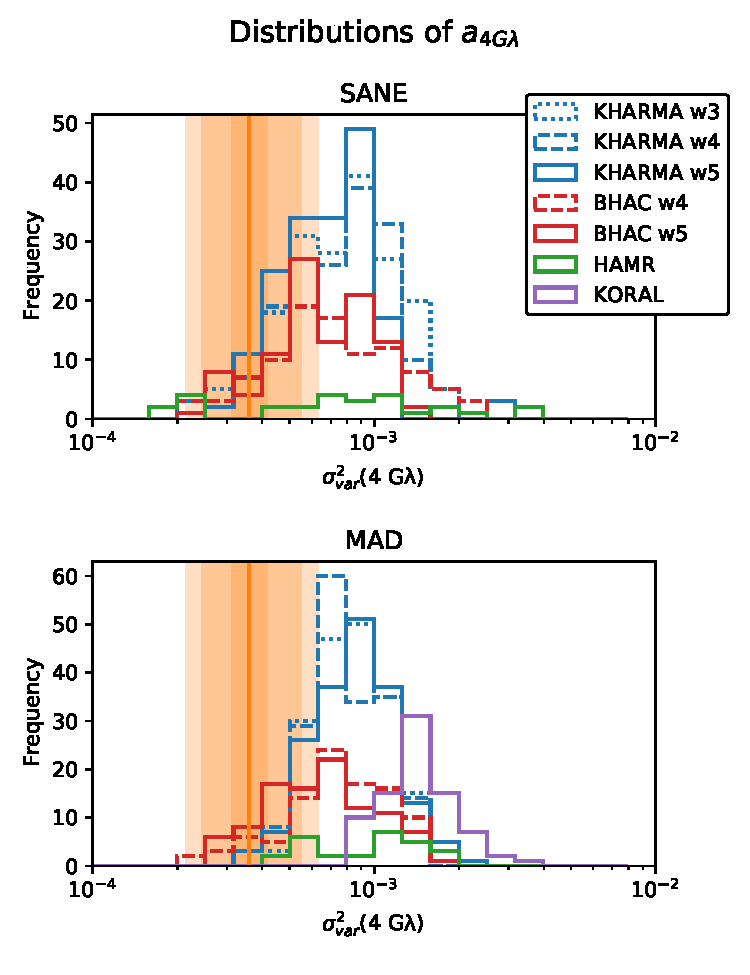
\includegraphics[width=\columnwidth]{./figures/va_hist.pdf}
%   \caption{Distributions of $PSD(4\,\mathrm{G}\lambda)$ for thermal models, compared to the observed distribution from the 2017 EHT campaign.
%   \dl{HAMR distribution will be updated later.}
%   \aeb{The quantity on the horizontal axis has been called $a_4$ in \citetalias{PaperIV}.  I have a similar concern regarding the abrupt end of the curves in this plot as well.  What do they mean?  How should these be interpreted?  There are the standard presentation issues (see \autoref{fig:sample_va}).}
%   \ckc{Nice new plot!  Are you using matplotlib fill\_between?  I suggest setting edgecolor to None and only set facecolor.  (Or setting linewidth=0 should also remove the lines in the orange shade.)}}
%   \label{fig:cmp_VLBI_var}
% \end{figure}

\begin{figure}
  \centering
  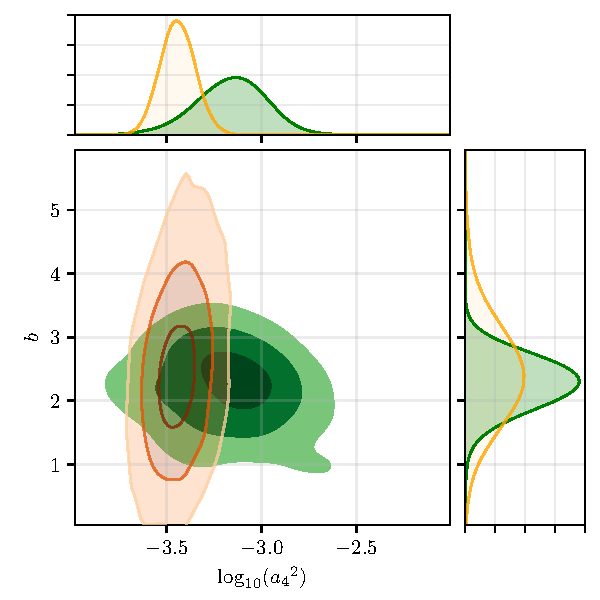
\includegraphics[width=\columnwidth]{./figures/grmhd_triangle_debiased_KHARMA.pdf}
  \caption{Distributions of $(\afour^2,b)$ for Illinois models (green), compared to the 2017 EHT observation (red). The distribution in $\afour$ for the Frankfurt models is slightly broader.}
  \label{fig:cmp_VLBI_var}
\end{figure}

% At a 1\% cut, the models that pass the PSD constraint also all pass the MI constraint. It should be noted that this is partially because these constraints are weakly correlated \dl{also partially because we're imposing constraints differently between VLBI and light curve, and the light curve constraint is more lenient} None of the 12 models with acceptable variability pass the other tests.

%------------------------------------------------------------------------------
\subsubsection{Summary of Constraints on Standard Models}

None of the standard thermal models (Frankfurt or Illinois) survive the full gauntlet of constraints.   Variability rejects about $70\%$ of models and prefers SANEs, which are quieter than MADs, while the remaining constraints prefer MAD models.
Evidently either (1) the models fail in some important respect, or (2) some of the data underlying the model tests are incorrect, or (3) one or more of the constraints have been misapplied.

We will discuss option (1) later.  To investigate options (2) and (3), we can ask what happens when we lift one constraint.  About 5\% of both the Frankfurt and Illinois model sets fail only 1 constraint.  For Frankfurt, 8 models fail only $\mi{3}$, and 2 fail only m-ring diameter.  For Illinois, 3 models fail only $\mi{3}$ and 5 fail only the 86\GHz size.  Suspicion therefore falls on $\mi{3}$, which rejects $\approx 70\%$ of Frankfurt and Illinois models.  Why might the $\mi{3}$ constraint be misleading?

\cfg{need learned commentary on the possibility of extended structure here.}

One possibility is that some fraction of the $230\GHz$ flux density, $f_{ext}$, is in an extended structure (a jet) that is slowly varying, captured in the ALMA light curves, and resolved out by EHT.  The implied $f_{ext}$ is model-dependent, but if $f_{ext} \sim 30\%$ then nearly all MAD models would pass $\mi{3}$ and many SANE models would be rejected as too quiet.  The $4$G$\lambda$ amplitude variability is normalized by the light curve and thus $a_4$ would increase by a similar factor.  Notice that if $f_{ext} > 0$ then the models would need to be re-normalized (the accretion rate adjusted) so that the compact flux is $(1 - f_{ext}) \times 2.4$Jy.  The extended flux hypothesis can be tested by the addition of new, short baselines to the EHT.

A second possibility is that physical or numerical errors in the models cause the variability to be overstated.  Several possibilities, including viscosity, radiative cooling, pair production, helium accretion, numerical resolution, simulation duration, and boundary conditions are discussed in Section \ref{sec:discussions}.  We will consider nonthermal eDF models, wind-fed models, and tilted models next.  None sharply reduce $\mi{3}$.

If $\mi{3}$ is set aside then 3 models survive from Frankfurt and Illinois.  All are MAD.  These are: $\abh = 0.5, i = 30, \Rh = 40$; $\abh = 0.5, i = 30, \Rh = 160$; and $\abh = 0.94, i = 10, \Rh = 160$.  These models are clustered in parameter space and pass 10 of 11 tests.  They explain most of the data.  We identify these as ``best-bet'' models in the discussion that follows.

%\begin{figure*}
%  \centering
%  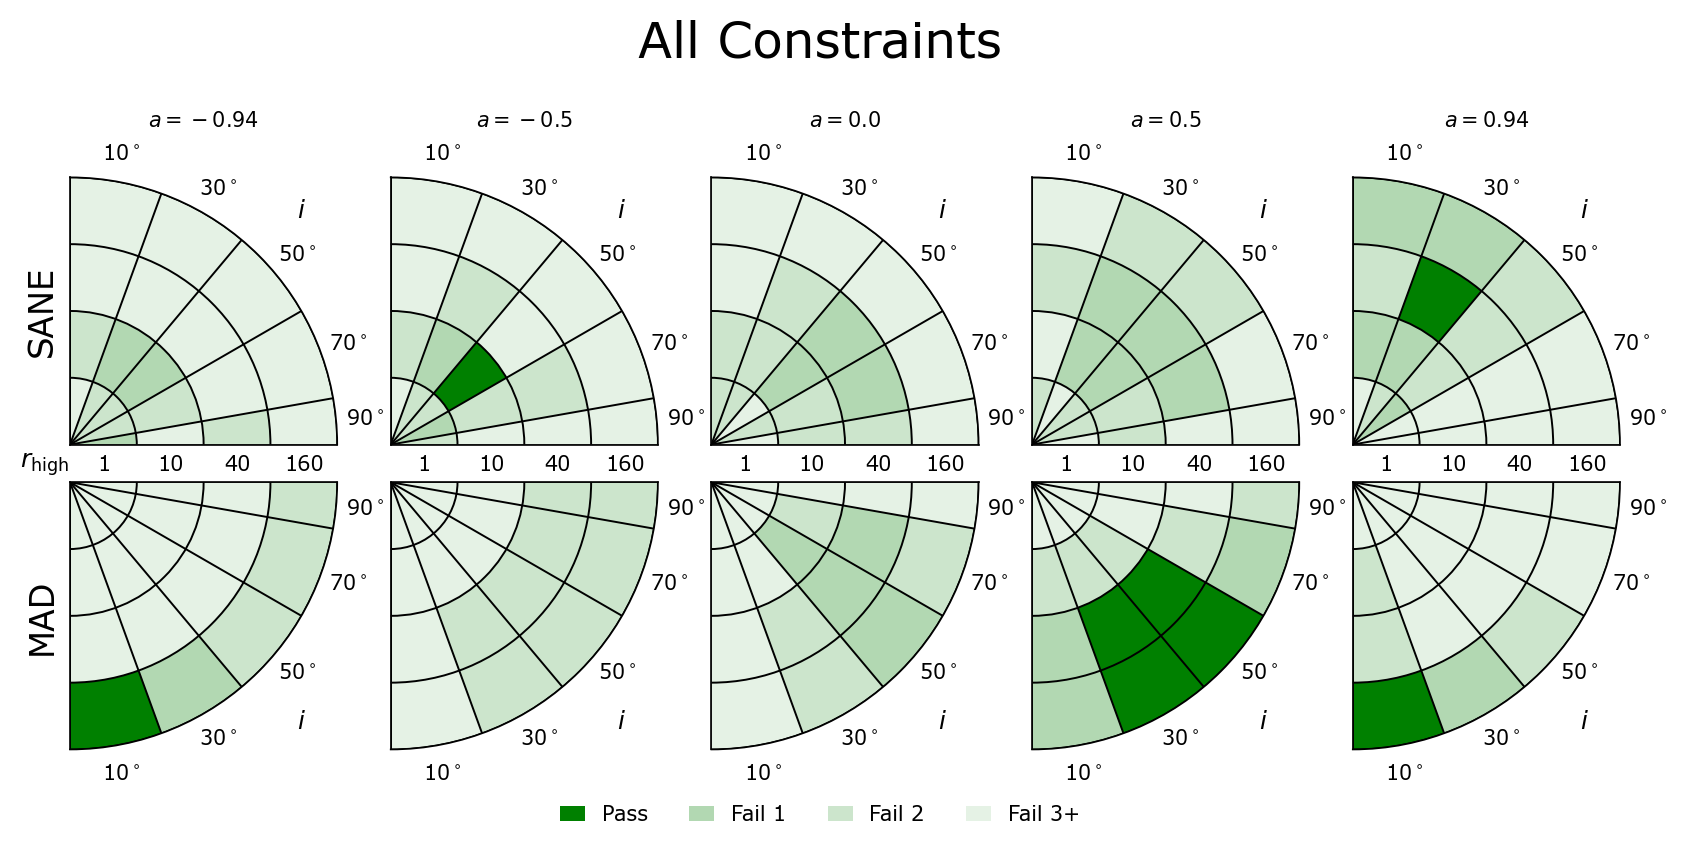
\includegraphics[width=\textwidth]{./figures/All_Constraints.png}
%  \caption{Combined EHT and non-EHT constraints, excluding variability.}
 % \label{fig:all_cuts}
%\end{figure*}

% this is now moved to appendix as discussed on Thursday Dec 9 2021 among coordinators
% %------------------------------------------------------------------------------
% \subsubsection{Inter-Model Comparison: $\Rh$ Thermal Models}

% % note: passfail tables are consistently, e.g., tab:illinoisPF or tab:VKhamrPF

% \subsubsubsection{Frankfurt Thermal $\Rh$ Models}

% As can be seen in Table \ref{tab:GRMHDmodels} the thermal models have been calculated for an identical parameter space from two different codes, namely KHARMA and BHAC for the GRMHD simulations and iPOLE and BHOSS for the GRRT calculations. This allows us for the first time to perform an in depth comparison between the different numerical methods used in this work in addition to the EHTC code comparison projects \citep{2019ApJS..243...26P,2020ApJ...897..148G}.

% \begin{figure*}
%   \centering
%   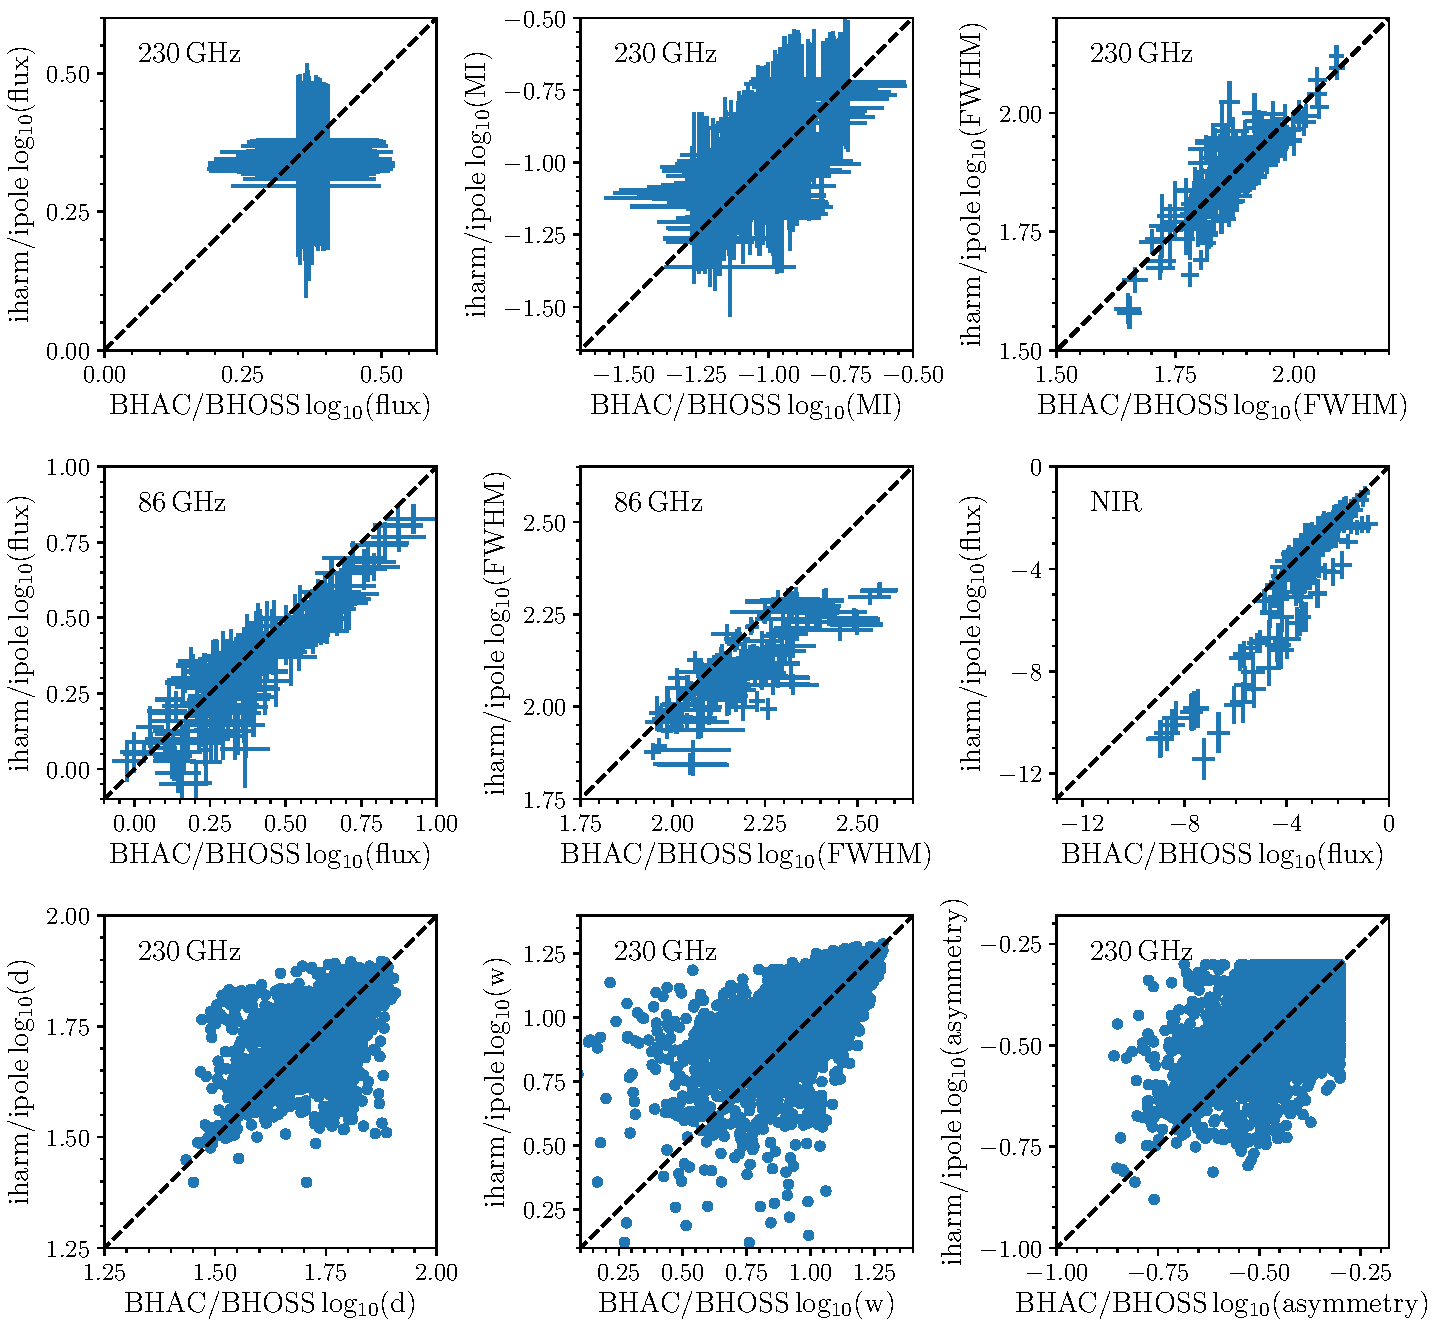
\includegraphics[width=0.8\textwidth]{./figures/BHAC_iharm_correlation}
%   \caption{Correlation between BHAC and KHARMA models for 9 model constraints.  The horizontal axis is the constraint value from \bhac/\bhoss, and the vertical axis shows the constraint value from \kharma/\ipole.  Each point corresponds to a single model, with the width of the distribution shown by the error bars.  See text for details.}
%   \label{fig:modelcorrelation}
% \end{figure*}

% In Figure \ref{fig:modelcorrelation} we show the correlation between the thermal KHARMA and BHAC models for constraints where we have predictions from both models.

% The top row shows from left to right the 230\GHz flux density, the 230\GHz modulation index, MI, computed for a time window of 3 hours, and the 230\GHz image size obtained from image moments. Since we normalise the 230\GHz images to an average flux of 2.4\,Jy within a time window of 5000\,M (corresponds to 28.5 h for SgrA a mass of $4.14\times 10^6\,\msun$), the scatter around this values is small. The deviation from an ideal correlation reflects the precision and number of GRMHD snapshots included during normalization procedure.

% The correlation in the 3\,hour modulation index spreads over $\Delta \mi{3}=0.75$ which serves as a measure of intra-code ( e.g., MAD vs. SANE accretion) and inter-code (BHAC vs. KHARMA) differences. Despite these differences the models show a strong correlation throughout the investigated models and parameter space.

% We found a strong correlation between models and codes for the image size computed from image moments, i.e. second moments analysis.

% \cfg{This may change if we recompute the major axis, etc., for the IL 86\GHz large fov images}
% The middle row presents the correlation plots for the 86\GHz flux density (left), the 86\GHz image size using second moments (middle) and the NIR flux (right). The 86\GHz flux and 86\GHz image size exhibit a shift toward larger values for the BHAC models. This difference can be explained by the larger field of view used for the BHAC models at 86\GHz during the radiative transfer calculations. Thus, more extended structure and therefore a larger total flux is included in the BHAC models. This affects mainly models with large inclinations $i\geq70^\circ$ and jet dominated emission models ($\rm{R}_{\rm high}\geq 40$).

% The NIR fluxes show a tight correlation over four orders of magnitude and systematically larger flux for the BHAC models for low NIR fluxes ($\log_{10}(NIR)<-7$). These fluxes are far below the NIR constraints of $\sim 1mJy$, and therefore they do not affect the passing or failing of the models. In the thermal models the NIR flux is generated from the tail of the electron distribution function and is thus very sensitive to the electron temperature. Small differences in the distribution and value of the electron temperature between the two codes explain the observed de-correlation at very low NIR flux.

% The correlation between models for the m-ring parameters is presented in the third row of Fig.~\ref{fig:modelcorrelation}. The correlation of the diameter of the m-ring is plotted in the left panel. The spread covers nearly the same extent as the 230\GHz image size (top row, right panel) however the scatter in the correlation is larger.  The same is true for the width of the m-ring (middle panel in the last row of Fig.~\ref{fig:modelcorrelation}). Compared to the diameter and width of the m-ring, the asymmetry of the m-ring is less correlated (right panel). Notice that horizontal and vertical limits in the asymmetries occur since the parameter hits the boundary of the allowed range.

% The smaller correlation of the m-ring parameters as compared to the other parameters presented in Fig.~\ref{fig:modelcorrelation} is a consequence of the noisy nature of the m-ring fits.  Still, the distributions are quite symmetric under reflection across the diagonal, so the models are at least not biased with respect to each other.  Notice also that these plots do not capture all the information that is contained in the distribution of m-ring parameters, just the central value.

% We find ourselves somewhat surprised by the strength of the correlations seen in Figure \ref{fig:modelcorrelation}.  The range of each constraint is significantly larger than the width of the correlation, so the variations between models are real, detectable, and reproducible with independent codes.  The question of the origin of the systematic offsets between models for some constraints (for example, in the NIR) is interesting but beyond the scope of this paper.

% \subsubsubsection{\hamr Models}

% %\note{Doosoo, Koushik to write here about HAMR thermal models.}
% Along the KHARMA/iPOLE and BHAC/BHOSS models, we produced a set of thermal models out to $35,000\tg$ using the GRMHD code H-AMR and the GRRT code BHOSS (see Table~\ref{tab:GRMHDmodels}). These models consider a gas adiabatic index of $\Gamma_{\rm ad}=5/3$ for the SANE models and $\Gamma_{\rm ad}=13/9$ for the MAD models (Table~\ref{tab:radiativemodels}), allowing us to understand how sensitive the images are to the GRMHD fluid properties, in addition to code numerics.

% We are glad to note that overall, the H-AMR/BHOSS thermal eDF images perform similarly to the KHARMA/iPOLE and BHAC/BHOSS models. \kc{needs verification from Michi}

% \kc{is the plan to do H-AMR and KHARMA correlations similar to figure 18?}

%\subsubsubsection{\koral Long Models}
% moved up to variability section
% We have also considered a set of thermal, $\Rh$, MAD models run with the \koral code out to $\sim 100,000\tg$.  These models permit us to assess the importance of integration time for application of the constraints.  They permit us to obtain more accurate distributions for the constraint quantites, and to assess whether the constraints evolve from the beginning to end of the integrations. We do not see evidence for evolution in the \koral  model set (a full pass/fail table is given in Appendix \ref{app:tables}, Table~\ref{tab:koralPF}). The \koral pass/fail results are similar to those for comparable models in the \kharma thermal model set. Moreover the constraints measured at the beginning of the evolution are similar to those measured at the end.

%==============================================================================
\subsection{Non-Standard Models}

We now turn to models that differ from the standard aligned, thermal, $\Rh$ based models.  These include aligned models that use a different scheme for assigning temperatures to a thermal eDF; aligned models with a power-law component or kappa component in the eDF; tilted models; and stellar wind-fed models.

%------------------------------------------------------------------------------
\subsubsection{Critical Beta Model}

First we consider the consequences of changing the $\Rh$ temperature assignment scheme in thermal models.  The $\Rh$ prescription has been the default parameterization.  Assuming that the ion-electron temperature ratio $R$ depends instantaneously on local conditions restricts the range of possibilities but still leaves a vast function space of alternative parameterizations.  A well-motivated choice is the critical beta model \citep{2020MNRAS.493.1404A}, which sets $T_e = f (T_e + T_i) \exp(-\beta/\beta_c)$.  This model has two parameters, $f$ and $\beta_c$; we consider a single point in the parameter space, $f = 0.5$, $\beta_c = 1$.

We have run all tests except X-ray for the critical beta models (NIR is calculated with imaging only and therefore does not include Compton scattering).  The full set of results is given in Appendix~\ref{app:tables}, Table~\ref{tab:betacritPF}.

To summarize, all critical beta models fail the non-EHT constraints, with 86GHz size constraint rejecting most models as too small.  The variability constraints fail $77\%$ of the models.  No models survive the combined EHT and non-EHT constraints, excluding variability.  This does not imply that critical beta models are ruled out, since we have only tested a single parameter set.

% cfg commented out 12 dec; edited down for consistency in style.

%to span the uncertainties in emitting particle thermodynamics in EHT analyses. The $\Rh$ models  are compatible with the well-motivated turbulent plasma heating ADAF models of \cite{1999ApJ...520..248Q} in asymptotic behavior of electron-to-total heating ratio as a function of plasma $\beta$. There is, however, a vast function space of possible alternative parameterizations. Here we have also considered the Critical Beta model \cite{2020MNRAS.493.1404A}, which sets $T_e = f (T_e + T_i) \exp(-\beta/\beta_c)$.  The model is motivated by the observation that when the transition between electron heating domination and proton heating domination is smoothed (controlled by increasing exponent parameter $\beta_c$), the 230\GHz emitting region profile tends to be less coronally dominated and more compact and asymmetric. This is a consequence, when fixing synthetic image flux, of higher critical beta values shifting the locus of electrons dominating the emission profile towards the colder, higher density equatorial inflow.  We consider only a single point in the critical beta parameter space, with $f = \beta_c = 1$. We have applied a subset of tests to the critical beta models (all except X-ray; NIR is calculated with imaging only and therefore does not include Compton scattering).  The full set of results is given in Appendix~\ref{app:tables}, Table~\ref{tab:betacritPF}. All Critical beta models with high inclinations fail EHT constraints, which is consistent with our main conclusion about the thermal models. We also find that all critical beta models fail all considered non-EHT constraints.

% CFG: we shouldn't report preliminary indications here
%A second motivation is that there are preliminary indications that the exponential electron cooling in the Critical Beta Model suppressed the SANE bremsstrahlung spectral component allowing more to pass the X-ray constraint.

%------------------------------------------------------------------------------
\subsubsection{Thermal Plus \texorpdfstring{$p = 4$}{p=4} Power-law Models}

So far we have assumed a thermal (Maxwell-J{\"u}ttner) eDF.  Next we assume that some electrons are accelerated to a non-thermal tail.  There are multiple ways of doing this, but we will continue to assume that the eDF depends instantaneously on local conditions and to set the accretion rate so that the time-averaged 230\GHz compact flux is 2.4 Jy.

% cfg 12-dec: we will comment this out by 13-dec unless we get more info, from here =>
First we employ a hybrid thermal/power-law tail distribution using \hamr/\bhoss, and assume a power-law index of $p=4$ with a constant non-thermal acceleration efficiency $\epsilon=n_{\rm e, power-law}/n_{\rm e, thermal}=0.1$. Following the method given in \citet{Chatterjee2021}, the power-law tail is stitched to the thermal core by choosing the minimum Lorentz factor limit of the power-law $\gamma_{\rm min}$ to be at the peak of the Maxwellian component. The upper end of the power-law is taken to $10^5 \gamma_{\rm min}$.  The temperature of the thermal component is set by the $\Rh$ prescription.  We find that the accretion rate is slightly smaller than for corresponding thermal models, suggesting that the power-law components contributes to the 230\GHz total intensity.

%..............................................................................
\subsubsubsection{230\GHz VLBI pre-image size}

Hybrid thermal/power-law models have similar 230\GHz VLBI pre-image sizes to their purely thermal counterparts. This is because the power-law index is large enough

%..............................................................................
\subsubsubsection{86\GHz flux}

In general, the $R_{\rm high}=1$ models produce too much 86\GHz flux. Since the lower limit of the power-law $\gamma_{\rm min}$ is directly affected by the local electron temperature, the highest energy electrons are located in the jet sheath where the ion and electron temperatures are similar, i.e. $T_i\approx T_e$. Indeed this is why SANE models produce more 86\GHz flux when non-thermal electrons are introduced, especially at larger $R_{\rm high}$ values. On the other hand, MAD pure thermal and mixed thermal/non-thermal models behave similarly as the bulk of the emission is produced in the inner disk.

%..............................................................................
\subsubsubsection{86\GHz image size}

...

%..............................................................................
\subsubsubsection{NIR constraints}

The addition of the power-law tail primarily increases the flux in the NIR and thus, the NIR GRAVITY flux of 1.0 mJy could provide a constraint on the power-law index and the acceleration efficiency. In brief, $R_{\rm high}=1$ and $40$ MAD models are ruled out by the NIR constraint.

%..............................................................................
\subsubsubsection{ALMA Light curves}

...

%..............................................................................
\subsubsubsection{m-ring}

\note{Razi to write here about variable kappa models.  Define a subsection, describe the results and how they differ from the thermal results.}\kc{might be better to move this to 4.2.3 along with bhac/bhoss results}

% cfg 12-dec: we will comment this out by 13-dec unless we get more info, to here <=

%------------------------------------------------------------------------------
\subsubsection{Constant kappa models with \texorpdfstring{$\kappa = 5$}{k = 5}}

Next we consider a model in which {\em all} electrons are in a kappa eDF, which has a thermal core and a power-law tail.  We set $\kappa = 5$ everywhere,  motivated by \cite{2016PhRvL.117w5101K}, who found $\kappa = 5$ to be a good fit to the ion DF in a 3D hybrid simulation of MHD turbulence.  The power-law tail then has $p = \kappa - 1 = 4$, and at high frequency $\nu L_\nu \sim \nu^s$ where $s = 2 - \kappa/2 = -1/2$.
\cmf{If not stated otherwise the width parameter $w$ of the kappa distribution (see Eq. \ref{eq:kappa}) is set by $w= (\kappa - 3) \Theta_e/\kappa$, where the dimensionless electron temperature, $\Theta_e$, is computed according to Eq. \ref{eq:rhigh_prescription}. The underlying GRMHD simulations are taken from the \bhac runs and we use the time window from 25\,kM to 30\,kM. The radiative transfer is done employing the GRRT code \bhoss and we created images every 50\,M using the same inclinations and $R_{\rm high}$ values as for the thermal models. Each model is individually normalized to an average flux of 2.4\,Jy at 230\GHz.}

%..............................................................................
\subsubsubsection{230\GHz VLBI pre-image size}

In the case of the MAD models the size of the $\kappa=5$ does not change. This can be explained by the fact that most of the emission is produced in the midplane. For the SANE models we find two different behaviors: The source size slightly increases for $R_{\rm high}<40$ and decreases for $R_{\rm high}\geq 40$ especially in for the positive black hole spins and high inclinations. In the SANE case the mass accretion rate decreases as compared to the thermal models indicating that particles from the tail of the kappa distribution contribute the 230\GHz flux. Increasing the $R_{\rm high}$ value the emission region is shifted from the midplane towards the polar region for the SANE models. Given that for the kappa distribution more emission is generated as in the thermal case the emission region becomes more compact. Together with the higher Doppler boosting at shorter distances from the black hole the source size decreases which explains the trend with black hole spin.

%..............................................................................
\subsubsubsection{86\GHz flux and Source Size}

The 86\GHz image size behave similar than the 230\GHz images.

%..............................................................................
\subsubsubsection{NIR constraints}

All MAD model generate more NIR emission than the 1.0\,mJy and thus fail the NIR constraints. Similar, the SANE models with $R_{\rm high}>1$ overshoot the NIR constraint.

%..............................................................................
\subsubsubsection{Light Curve Variability}

The $\mi{3}$ constraint is computed for a time window of length 5000\,$\rm{GM/c^3}$. This window is a factor three shorter than for the thermal models and thus a direct comparison cannot be performed. However we find that 66\% of the models fail this test. The number roughly agrees with the thermal models and thus we conclude that the non-thermal particles included via a kappa eDF with $kappa=5$ does not affect the variability.

%..............................................................................
\subsubsubsection{M-ring Constraint}

\note{to be done}

% cfg 12-dec: this section will be commented out soon unless we receive more results

%performed 3D kinetic numerical simulations of accretion disks and found that the distribution of the ions is well described by kappa distribution with $kappa=5$. We adopted this results and assume that the radiating electrons follows a similar distribution as the ion. Therefore, we performed radiative transfer calculations using a kappa distribution with fixed value of $\kappa=5$.
%\newline \cmf{more details tomorrow: all MAD models overshoot the the NIR flux limit and only a few SANE models are below flux threshold. The SANE models which pass the NIR constraints produce too large 86\GHz images}

%==============================================================================
\subsubsection{Mixed Thermal/Kappa Model}

Next we consider a mixed thermal/nonthermal eDF, with the nonthermal component following the kappa DF with $\kappa = 3.5$.  At high frequency $\nu L_\nu \sim \nu^s$ with $s = 2 - \kappa/2 = 1/4$, similar to what is seen in NIR flares \citep{2007ApJ...667..900H}.  For this model set the GRMHD models use \bhac and the imaging uses \bhoss.

The fraction of nonthermal electrons is assumed to depend on $\sigma$ and $\beta$.  We write the emissivity as:
\begin{equation}
j_{\nu,\rm{tot}}=(1-\epsilon) j_{\nu,\rm{thermal}} + \epsilon j_{\nu, \kappa},
\label{eq:kappaeff}
\end{equation}
where the nonthermal efficiency $\epsilon( \varepsilon, \beta, \sigma)$ is
\begin{equation}
    \epsilon(\varepsilon,\beta,\sigma)=\varepsilon\,
    \left[1 - e^{-\beta^{-2}}\right]
    \left[1-e^{-(\sigma/\sigma_{\rm min})^2}\right].
    \label{eq:efficiencybetasigma}
\end{equation}
An example time- and azimuth-averaged distribution of $\epsilon$ is shown in Fig. \ref{fig:varepsilon}.  Evidently $\epsilon \rightarrow 0$ in the disk while $\epsilon \rightarrow \varepsilon$ in the jet.  Since we remove emission at $\sigma > \sigma_{\rm cut} = 1$ the non-thermal electrons are confined to the jet sheath.

We set $\sigma_{\rm min}=0.01$ and vary the base efficiency, $\varepsilon$ over 0.05, 0.1 and 0.2.  At each $\varepsilon$ we generate a model set spanning the same parameter space as the thermal models (see Table \ref{tab:radiativemodels} for details),
and normalize the accretion rate using the standard procedure (see Section \ref{sec:models}.

%For each model we iterate the mass accretion rate to obtain an average flux of 2.4\,Jy at 230\GHz across a time interval of 5000\,M. In order to explore several values of $\varepsilon$ efficiently we increased the model snapshot cadence to 50\,M. This allows us to keep the numerical costs for this parameter sweep low while still being within the correlation time of the GRMHD simulations.
%($t_{\rm corr}\approx 50-100\,M$) \cmf{ do we have reference for this? So far this result is not published, maybe Boris paper?}.
% CFG: this is mentioned earlier in the paper and also implicit, but not actually calculated, in Boris's paper.  Let us not specify a correlation time here, so that we don't set the correlation time in multiple places.

%An example of the distribution of the efficiency can be seen in the right half of  Fig. \ref{fig:varepsilon}. The efficiency quickly $\epsilon=0$ within the disk region while within the jet the efficiency reaches the defined base-efficiency. Thus (and as usual removing emission at $\sigma > \sigma_{\rm cut}=1$) the non-thermal particles are mainly located in jet sheath.

\begin{figure}[t!]
  \centering
  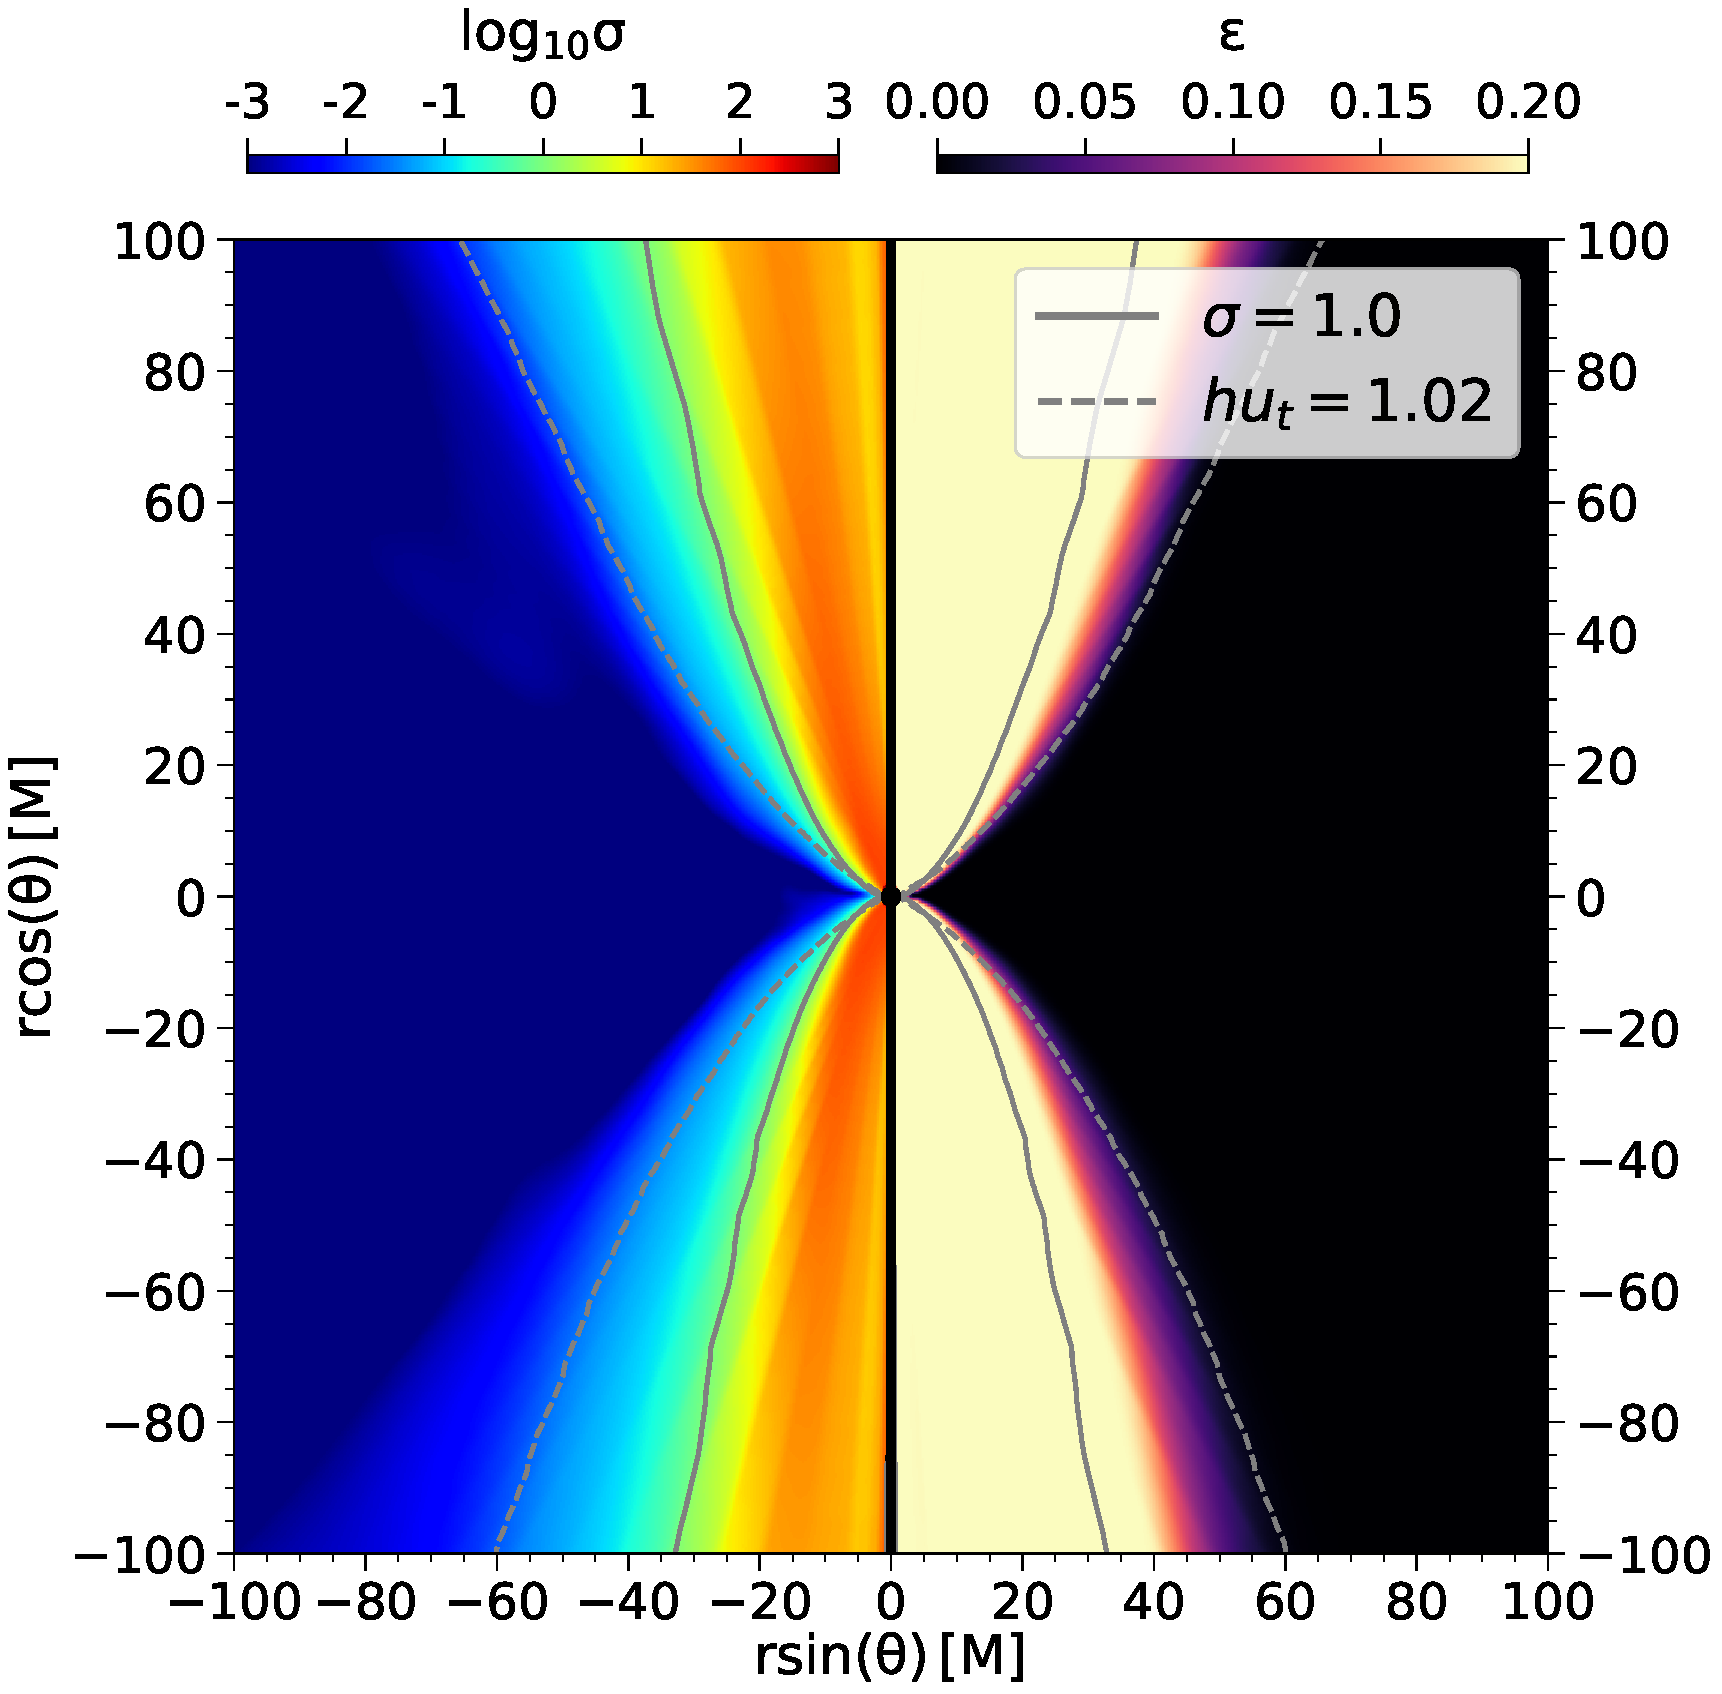
\includegraphics[width=\columnwidth]{./figures/GRMHDphiavera0.94sigmaeta.pdf}
  \caption{Time and azimuthal averaged distribution of the magnetization, $\sigma$ (left half) and the efficiency, $\epsilon(\varepsilon,\beta,\sigma)$ using $\varepsilon=0.2 $ for a \bhac MAD GRMHD simulation with $\abh=0.94$. The solid gray line corresponds to $\sigma=1$ and the dashed line indicates out-flowing plasma via the Bernoulli parameter ($-h u_{t}>1.02$).
  \ckc{Should we move this figure to the model section, as a way to demonstrate how the GRMHD and eDF look like?}}
  \label{fig:varepsilon}
\end{figure}

%In the following we will elaborate on the impact of adding non-thermal particles via the kappa electron distribution with fixed kappa value ($\kappa=3.5$) and three different base efficiencies $\varepsilon=$0.05, 0.1 and 0.2 on the observational constraints listed in Section~\ref{subsec:thermal}.

%..............................................................................
\subsubsubsection{230\GHz VLBI pre-image size}

The addition of non-thermal particles produces almost undetectable changes in the 230\GHz VLBI pre-image sizes for the MAD models and a minor effect for the SANE models.

For MADs, independent of $\Rh$, $230$GHz emission is mostly produced in the disk region (see \citetalias{M87PaperV} and Fig.~8 in \citealt{Wong_2022} for a 3-D rendering).  Increasing $\Rh$ will therefore not push the emission region into the jet where the non-thermal particles are located and thus their contribution to the total emission structure is negligible.

For SANEs, models with $\Rh>40$ exhibit a minor increase in the source size.  Increasing $\Rh$ in SANE models pushes the emission toward the jet sheath, but the effect is minor because most of the emission is still produced by thermal electrons with temperature set by the $\Rh$ prescription.

%An increase in $\Rh$ suppresses the emission from particles in the disk (by decreasing the electron temperature) and thus enhances emission from jet.  Since most the non-thermal particles are located in the sheath of the jet their impact on the source size is largest if the bulk of the thermal emission is also produced there.

% CFG: this is confusing.  is it needed?
%In addition the thermal synchrotron emissivity decreases at high frequency as $j_{\nu}\propto \exp{\left(-(\nu/\nu_c)^{1/3} \right)}$ while for the kappa distribution as $j_{\nu}\propto \nu^{-(\kappa -2)/2}$. This implies that for the same electron temperature the non-thermal flux is compared to a thermal one higher and thus leads to a more extended jet structure for the models including non-thermal particles.

%In MADs, independent of the choice of $\Rh$, the emission is mostly produced in the disk region (see \citetalias{M87PaperV} and Fig.~8 in \citet{Wong_2022} for a 3-D rendering).  Increasing $\Rh$ will not push the emission region into the jet where the non-thermal particles are located and thus their contribution to the total emission structure is negligible.

%..............................................................................
\subsubsubsection{86\GHz Flux and Source Size}

% cfg 12-dec: this has already been mentioned elsewhere
%The 86\GHz GMVA+ALMA observations
%probe a larger field of view than the 230\GHz EHT observations, so we increased the field of view for the 86\GHz to 800\,$\rm{\mu as}$ during the radiative transfer calculations. Again the non-thermal particles are mainly located in the jet sheath and thus the increased field of view ensures that no extended flux is missing during the comparison with the 86\GHz observations.

The 86\GHz flux density for both SANE and MAD models is unaffected by the addition of non-thermal particles.  There is a small effect for SANE models with $\Rh>40$, but even for $\varepsilon = 0.2$ this does not change which models are rejected.  Similarly the 86\GHz major axis FWHM is unaffected by the addition of non-thermal particles.

%n case of the SANE models the edges of the 86\GHz flux distribution are slightly shifted in the case of $\Rh>40$. However, including non-thermal particles even with the highest base efficiency $\varepsilon=0.2$ does not change the scoring of a model, i.e., a thermal-only model which full-fills the 86\GHz constrain is still accepted if non-thermal particles are included.

%This behaviour can be explained by the fact that the bulk of the emission in both accretion models is generated in with a few gravitational radii. Since the non-thermal particles are mainly located in the jet sheath and thei ratio between non-thermal to thermal particles is at most 20\% the contribution of the non-thermal particles to the 86\GHz flux can be neglected.

%..............................................................................
%\subsubsubsection{86\GHz image size}

%The behaviour of the 86\GHz image size is very similar to the above described 230\GHz image size: There is no change in image size for the MAD models and only a minor increase in the SANE models for $\Rh>40$. The physical reasons for this behaviour follows the same arguments as in the 230\GHz VLBI pre-image size.

%..............................................................................
\subsubsubsection{NIR constraints}

The addition of non-thermal electrons increases the NIR flux for all models. For SANE models, except $\Rh=1$, the addition of non-thermal particles leads to over-production of NIR. For MAD models, all models over-produce NIR for $\varepsilon \ge 0.05$.

% commented out 12-dec, cfg: we should show trends in some model and some test other than this one, since we can easily make the case that the NIR increases as $\varepsilon$ increases.
%\begin{figure*}
%  \centering
%  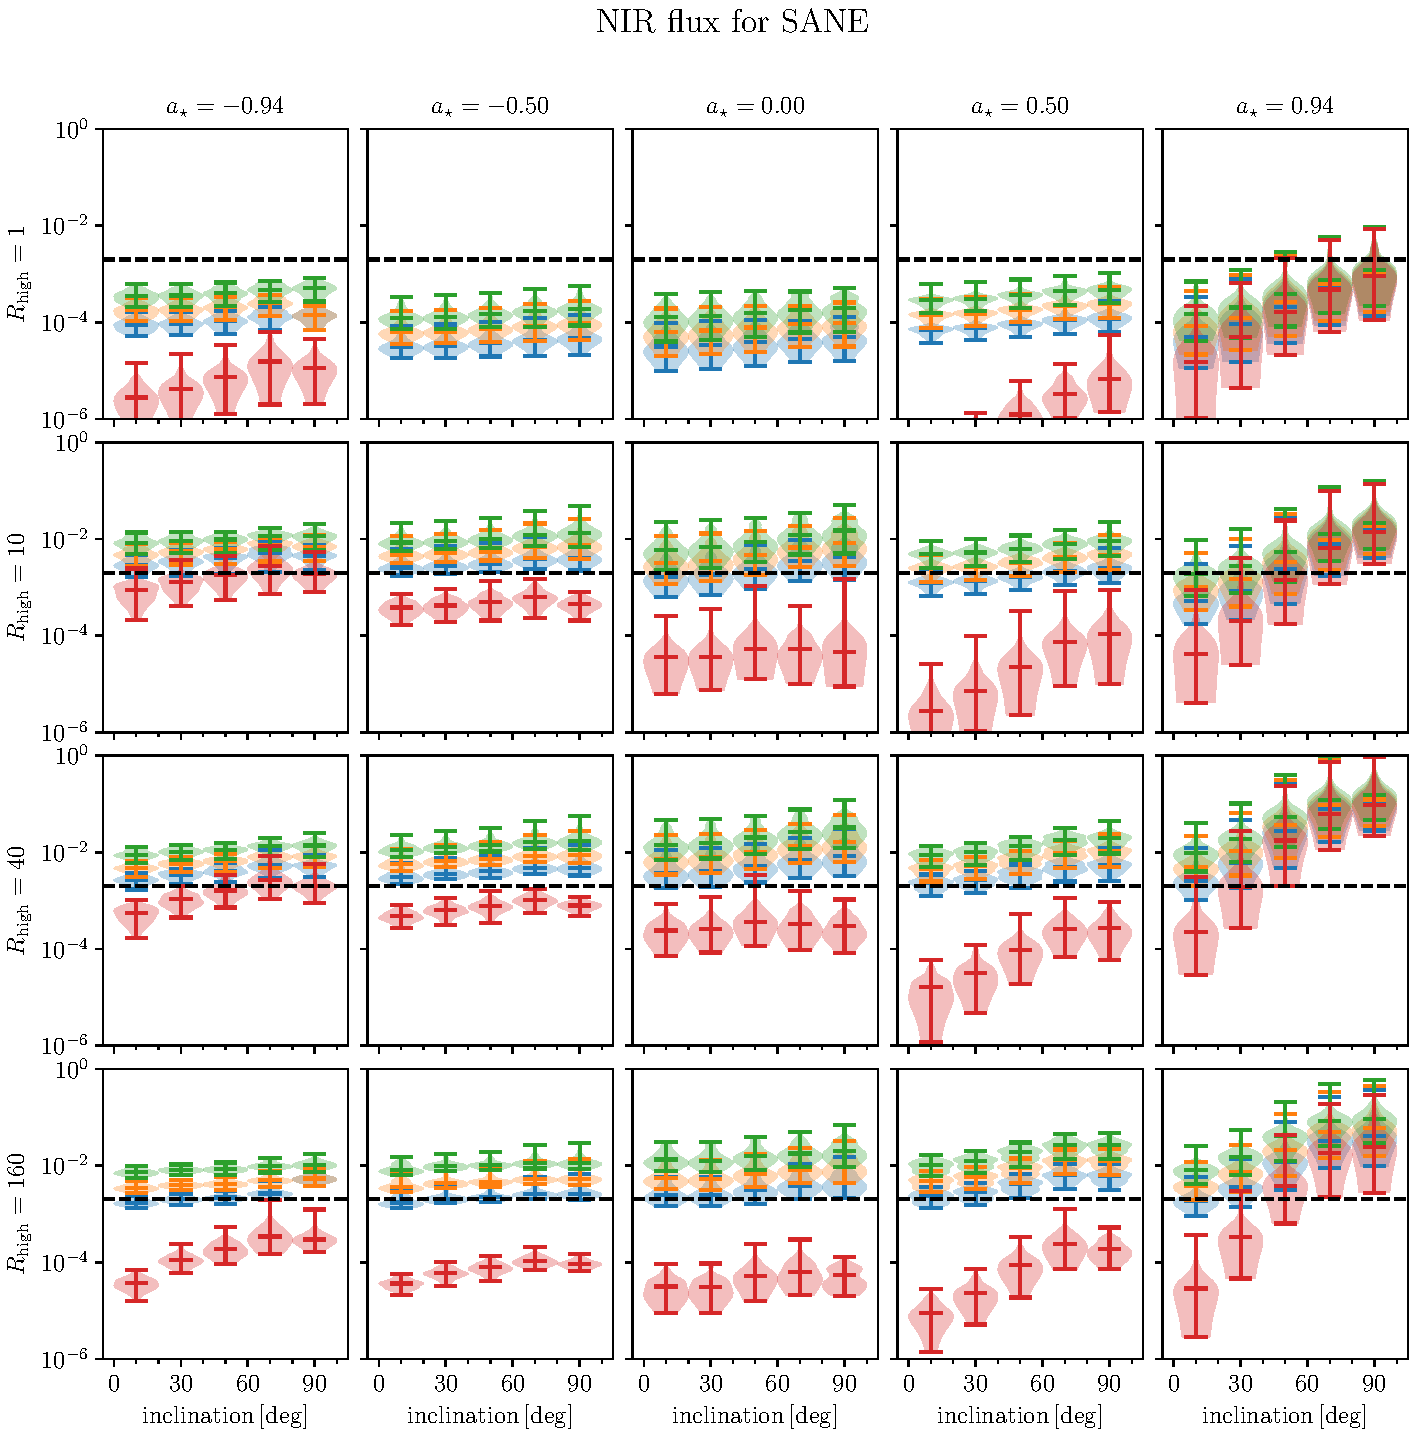
\includegraphics[width=0.8\textwidth]{./figures/SANE_NIR_standard.pdf}
%  \caption{Impact of non-thermal electrons on NIR flux constraint for the \bhac/\bhoss variable nonthermal efficiency model. NIR flux distributions are shown for SANE accretion models with thermal and non-thermal eDF with fixed $\kappa=3.4$ and $\epsilon\left(\sigma,\beta,\varepsilon\right)$ defined by Equation~\ref{eq:efficiencybetasigma}. The red violin plots correspond to a thermal eDF, blue, orange and green indicate kappa eDF with $\varepsilon=$0.05,0.1 and 0.2. The horizontal dashed line is the observational constraint.}
%  \label{fig:NIR_kappaepsilon}
%\end{figure*}

As noted above, NIR emission is produced from the tail of the eDF.  The thermal eDF tail decreases exponentially, while the kappa eDF tail decreases as a power law, so the increase in NIR flux density is unsurprising.  This is a general feature of the nonthermal models: NIR observations sharply limit the allowed population of nonthermal electrons.

%..............................................................................
\subsubsubsection{Light Curve Variability}

We compute $mi{3}$ for a window of $\num{5000}\tg$.  Notice that this is shorter than the standard models, which as three $\num{5000}\tg$ windows, so the results are less constraining.  The $\mi{3}$ test rejects about 1/2 of models for $\varepsilon = 0.05$, $0.1$, and $0.2$.  We conclude that $\varepsilon$ has no effect on the $\mi{3}$ test.

%For the comparison with the ALMA light curves we compute the modulation index for a 3\,hour time window and across the entire simulated time window of 28\,hours (5000\,GM/c$^3$). Similar to the 86\GHz flux the 230\GHz flux is mainly produced within a few gravitational radii and thus not affected by the addition of non-thermal particles using Eq. \ref{eq:kappaeff}. As in the previous constraints, the MAD accretion models are insensitive to the addition of non-thermal particles whereas the SANE models show some increased modulation index for $\Rh>40$. However, the distributions for thermal and non-thermal eDF are still largely overlapping.

%..............................................................................
\subsubsubsection{M-Ring Constraint}

The m-ring fitting is applied to the 230\GHz images. As mentioned earlier the flux and size of the 230\GHz images are not affected by the inclusion of non-thermal particles with fixed kappa and variable efficiency. Thus, we do not expect any changes in the distribution of the m-ring parameters.  Applying m-ring fitting to non-thermal models and a detailed comparison with the thermal results confirmed our initial assumption.

%\cmf{based on the results of Kotaro, who run the m-ring on non-thermal models}

%%%%%%%%%%%%%%%%%%%%%%%%%%%%%%%%%%%%%%%%%%%%%%%%%%%%%%%%%%%%%%%%%%%%%%%%%%%%%%%
% This table is for the feature model section
\begin{deluxetable*}{cccccc}
  \tablewidth{\textwidth}
  \tabletypesize{\footnotesize}
  \renewcommand{\arraystretch}{1.1}
  %
  \tablehead{%
    \colhead{Model}             &%
    \colhead{Spin $\abh$}       &%
    \colhead{Magnetization}     &%
    \colhead{eDF type}          &%
    \colhead{Temp. ratio $\Rh$} &%
    \colhead{Inclination $i$}    %
  }
  \startdata
  A & 0.94 & SANE & thermal                      &  40 & $30\degree$ \\ % Frankfurt
  B & 0.5  & MAD  & thermal                      &  40 & $30\degree$ \\ % Illinois
  C & 0.5  & MAD  & nonthermal variable $\kappa$ & 160 & $30\degree$    % HAMR
  \enddata
  %
  \caption{List of feature models that sample the more possible regions
    of the model parameter space.
    As Figure~\ref{fig:bestbets} shows below, these models broadly
    agree with the observation constraints, although they are not
    necessary the best fit models because of both observation and
    modeling noise.
    See Section~\ref{sec:bestbets} for detailed descriptions of these
    models and Section~\ref{sec:discussions} for discussions.}
  \label{tab:bestbets}
\end{deluxetable*}

%------------------------------------------------------------------------------
\subsubsection{Variable Kappa Model}

%\cfg{could we avod the equation and simply provide a reference and enough detail that someone could reproduce it?}\aco{What about inline equations?}

An alternative procedure for assigning a nonthermal eDF uses the  kappa model \eqref{eq:nonthermaleDF}, and sets $\kappa$ and $w$ according to \cite{2018ApJ...862...80B}, who model the effects of particle acceleration in magnetic reconnection.  In particular, we set
\begin{align}
  \kappa &= 2.8 +0.7\sigma^{-1/2} + 3.7\sigma^{-0.19}\tanh{(23.4\sigma^{0.26}\beta)}, \label{eq:kappa}\\
  w      &= \frac{ \kappa -3 }{\kappa} \Theta_e +
  \frac{\varepsilon}{2}\Big[1+\tanh(r-r_{\rm inj})\Big]\frac{\kappa - 3}{6 \kappa} \frac{m_p}{m_e} \sigma.
\end{align}
Evidently $w$ contains a thermal and nonthermal contribution, with the nonthermal contribution proportional to the nonthermal particle acceleration efficiency $\varepsilon$  \citep{2019A&A...632A...2D, 2021NatAs.tmp..218C}.  The thermal width $\Theta_e$ is set using the $\Rh$ prescription.

We set $\varepsilon=0$ and injection radius $r_{\rm inj}=10r_{g}$ following previous studies.  Nonzero $\varepsilon$ increases the averaged NIR flux by two orders of magnitude as $\varepsilon$ goes from 0 to 1, causing all models to overshoot NIR constraint.  Setting $\varepsilon \ne 0$ also causes the 86\GHz flux density and image size to increase \citep{2021arXiv211102518F}.

We use the emissivity and absorptivity, computed numerically for the interval $3 < \kappa \le 8$, from  \cite{2016ApJ...822...34P}. For $\kappa > 8$ we substitute a thermal eDF.  As in the standard models we turn off emission at $\sigma > 1$ (see Figure~\ref{fig:varepsilon}).

\cfg{need very brief discussion here of the codes and run durations}

\cfg{this section needs to incorporate both the \hamr and \bhac variable kappa models}

%..............................................................................
\subsubsubsection{86\GHz Major Axis}

We found that the 86\GHz image size is similar to the thermal and variable efficiency models, differing only for non-spinning black holes, where we have low magnetization, weak jet. As a consequence our prescription makes $\kappa$ large and the radiative properties of the plasma similar to those of a thermal eDF.
eDF with variable kappa power-law reduces to thermal distribution and the size of the image is a bit smaller than in thermal case. For $a_{\star}=0$ almost all SANE models pass the size constraint, $R_{\rm high}=1$ we have a bit larger image. For MAD $R_{\rm high}=40$ and $a_{\star}=0.94$, and cases for $R_{\rm high}=160$ and $a_{\star}=0.50$ we have a bit smaller size image than thermal case passing the constraint.

%..............................................................................
\subsubsubsection{86\GHz flux}

The total flux on overall non-thermal models increases in comparison to thermal models, however, the general results for MAD models do not change. For SANE models with R$_{\rm high}=1$ slightly increases, all of them fail in contrast with thermal models. While for $R_{\rm high}=10,40,80$ and $R_{\rm high}=160$ the flux decreases under the lower bound $1.8 \rm {Jy}$.

%..............................................................................
\subsubsubsection{NIR constraints}

The contribution of non-thermal electrons at the NIR emission produce larger flux in all models, independent on black hole spin, inclination angle or electron temperature. For MAD accretion models with $a_{\star}=0$ and $R_{\rm high}=1$ only small inclination $i=10^{\circ}$ pass the constraint. While models with $R_{\rm high}=10,40$ overshooting GRAVITY mean flux, again for thermal case these models satisfy the constraint. On the other hand, since for non-spinning black hole the jet is no well developed and the magnetization is low, for only  $R_{\rm high}=80$, $a_{\star}=0.5$ and $30^{\circ} \leq i$ survive, similar behavior for $R_{\rm high}=160$ and spins $|a_{\star}|=0.5$.
Larger emission than thermal models excludes SANE models for $R_{\rm high}=10$ and $\abh < 0$ as well as  $R_{\rm high}=40,~80$ and $\abh \leq 0.0$. While even larger NIR flux the models for $R_{\rm high}=160$ are still under the threshold.

%..............................................................................
\subsubsubsection{ALMA Light curves}

We compute the the modulation index  of the light curves of variable kappa models by discretizing the entire window of GRMHD simulations, $\rm 5000\,\tg$ ($\rm 28\,hours$) every $\rm 3\,hour$ (see Table \ref{tab:GRMHDmodels}). Similar to variable efficiency models, the non-thermal particles with variable kappa has not big impact on the flux at 230GHz. The behavior of modulation index and total flux for MAD accretion models are same as thermal, and variable efficiency eDFs. We found sightly high modulation index for $R_{\rm high}=1$ and $30^{\circ} \leq i$ for SANE accretion models, the models for $R_{\rm high}=80$ has same trend as $R_{\rm high}=40$.

%..............................................................................
\subsubsubsection{M-Ring}

%\aco{First Draft ... please add missing references ... waiting for calculations with help from Michi, Ben, Ck and Kotaro}\\

...

%..............................................................................
\subsubsubsection{Null Location}

...

%------------------------------------------------------------------------------
\subsubsection{Summary of Constraints on Non-Thermal Models}

The nonthermal eDF models considered here produce surprisingly little change compared to the thermal models for most constraints.  The 86 Ghz size and flux, which are the most important non-EHT constraints, are not detectably affected by the addition of nonthermal electrons.  The 230GHz m-ring fits are hardly affected at all by the addition of nonthermal electrons.  And $\mi{3}$ is also not detectably affected by the addition of nonthermal electrons.  The NIR flux density, however, is consistently increased by the nonthermal eDF prescriptions considered here.  In a large fraction of models this leads to overproduction of NIR.

%The effect of adding non-thermal electrons in a kappa eDF with  $\kappa=3.4$ and variable efficiency via Eq.~\ref{eq:efficiencybetasigma} can be summarized as follows:
%\begin{itemize}
 %   \item The 86\GHz and 230\GHz constraints are hardly affected by the addition of non-thermal particles.
%    \item Even the lowest base efficiency considered, $\varepsilon=0.05$, leads to an over-production of NIR flux. \cmf{indication that we need very localised regions of non-thermal particle productions and no "global" approach?}
%\end{itemize}

The effect of adding nonthermal electrons in a variable kappa eDF can be summarized as follows:

The effect of adding nonthermal electrons in a variable kappa eDF can be summarized as follows:

The effect of adding nonthermal electrons in a constant-kappa model can be summarized as follows:

The effect of adding nonthermal electrons in a power-law can be summarized as follows:

Most of our nonthermal models assign a width to the nonthermal component that depends on the an electron ``temperature'' assigned through the $\Rh$ scheme, so they are not fully independent of $\Rh$.

The nonthermal models are run for only $5000\tg$, so most  constraints can not be applied as precisely.  For example, the model distribution of $\mi{3}$ contains only $9$ points and correspondingly more uncertain.  It is therefore difficult to detect subtle changes in models.

%%%%%%%%%%%%%%%%%%%%%%%%%%%%%%%%%%%%%%%%%%%%%%%%%%%%%%%%%%%%%%%%%%%%%%%%%%%%%%%
% This figure is for the best-bet model section
\begin{figure*}
  \centering
  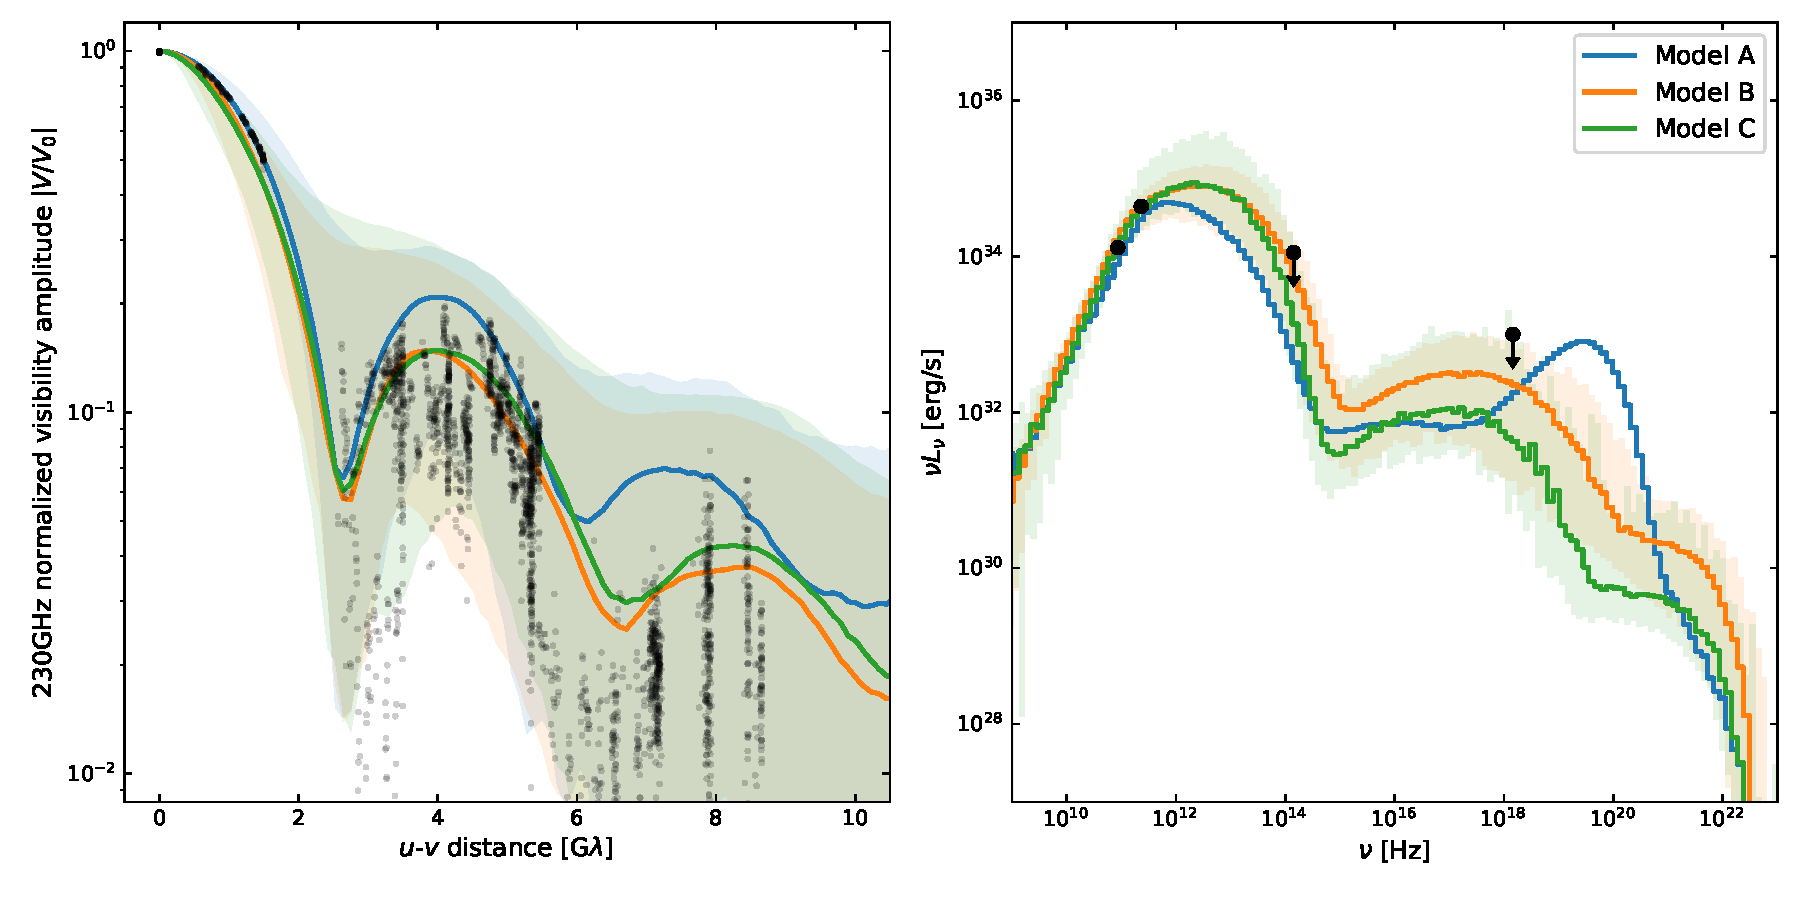
\includegraphics[width=\textwidth]{figures/bestbets.pdf}
  \caption{The visibility amplitudes and SEDs of the three feature
    models compared with data.
    In both panels, symbols in black are from observations; blue,
    orange, and green are Models~A, B, C, respetively (see
    Table~\ref{tab:bestbets} for definitions).
    (\emph{Left}) We show the visibility amplitudes as function of
    $(u, v)$ distance similar to Figure~\ref{fig:passfail_va}.
    For the observation data, we plot 10\sec incoherent averaged data
    from the HOPS pipeline on \aprilvii.
    For the models, the solid curves are the VAs for only the position
    angle $0\degree$ (parallel to the spin axis) for a particular
    snapshot.
    while the transparent bands show the 1 to 99 percentiles for all
    position angles and all time.
    This panel shows that the feature models agree well with the EHT
    VLBI data.
    (\emph{Right}) We show the SEDs for the feature models and again
    compare them with the observation constraints.
    The solid lines are the mean SEDs, while the transparent bands
    show the range across different snapshots.}
  \label{fig:bestbets}
\end{figure*}

%==============================================================================
\subsection{Tilted Models}

The aligned models considered up to now are a special case: in general one would expect that the spin angular momentum of the black hole and the orbital angular momentum of the accretion flow would be misaligned.  Here we consider misaligned flows around an $a_*=15/16$ black hole from \citet{Liska2018} and \citet{Chatterjee2020}.

All aligned models considered so far produce either a SANE or MAD accretion flow.  The tilted disk model initial conditions, however, produce a strongly magnetized but not MAD outcome, a state known as INSANE.  We consider three GRMHD models with tilt $0^{\circ}$, $30^{\circ}$ and $60^{\circ}$.

The tilted models exhibit a warped disk due to the Lense-Thirring torques imposed by the black hole.  The time-averaged disk and jet are therefore non-axisymmetric.
%Notice that the jets are always approximately perpendicular to the outer disk in these models.
Since the inner and the outer disk have different orientations, it is necessary to specify the coordinate axis of the observer.  We consider three  observer inclinations with respect to the {\em outer} disk at a single azimuth of $0\degree$ \citep[for more details, see][]{Chatterjee2020}.\footnote{A full parameter survey would run over azimuth angle as well.}  A full listing of the pass/fail results are given in Appendix~\ref{app:tables}, Table~\ref{tab:ThamrPF}.

The 230\GHz pre-image size of edge-on large $\Rh$ images increases slightly for the tilt-$60\degree$ compared to the aligned case. This occurs because the inner jet is warped and creates an extended image. This effect is also seen in the 86\GHz image size. On the other hand, the 86\GHz flux varies little with tilt despite the presence of a boosted jet component at large tilt angles.

% cfg 12-dec this is a testable proposition
%This suggests that, on average, most of the total flux at 230 and 86\GHz comes from a few gravitational radii from the black hole where the relativistic Doppler boost have comparable values between the in-going accretion flow and the out-flowing jet.

Variability increases wth tilt. In tilted disks, accretion occurs via thin plunging streams \citep[e.g.,][]{Fragile2007} where electrons in the shocked flow can be heated to relativistic temperatures \citep[e.g.][]{Dexter2013}, forming localized, fluctuating hotspots more easily than in aligned disks, thereby increasing flux variability \citep{Chatterjee2020}.

\cfg{Statement about which models pass and fail MI}

NIR flux also increases with tilt.  The NIR flux exceeds the 1.0 mJy limit for all 3 tilts, with a few exceptions, e.g. $R_{\rm high}=160$ models at $10^{\circ}$ inclination, which makes it difficult to favor the aligned case over the tilted one. Further, the presence of misalignment destroys the axisymmetric nature of the accretion flow.  The current model set covers a small parameter space in inclination and $R_{\rm high}$.  A thorough exploration of the source azimuthal angle with respect to the observer is left to future studies.

To summarize: for the model set considered here tilt primarily affects variability and the NIR flux density, increasing both and thus shifting acceptable aligned models into rejected models as tilt angle increases.

%==============================================================================
\subsection{Stellar Wind Fed Models}

The accretion models of \cite{2020ApJ...896L...6R, 2020MNRAS.492.3272R, 2018MNRAS.478.3544R} track plasma from  magnetized stellar winds down to the event horizon and provide a self-consistent picture of the origin of both gas and magnetic fields in the accreting plasma in \sgra.  The resulting inflow does not fully circularize, so the models also provide a distinct alternative to the standard models, which {\em assume} that the SANE or MAD initial conditions relax to a astrophysically accessible state for the inner accretion flow.

We consider two versions of the model: one in which the stellar wind magnetization is low ($\beta = 10^6$) and another and a second in which the magnetization is high ($\beta = 10^2$). $\Rh$ is adjusted until each model has the observed time-averaged 230\GHz flux density, with $\Rh = 13$ ($\beta = 10^6$) and $\Rh = 28$ ($\beta = 10^2$).

Both wind-fed models fail the m-ring width test, producing a width that is too small.  In addition both fail the 86GHz flux test: the 86GHz flux density is too large.  The wind-fed models also fail the $\mi{3}$ test, although they are quieter than MAD models and close to the cutoff.   All scoring results are given in Appendix~\ref{app:tables}, Table \ref{tab:resslerPF}.

Both non-EHT and EHT constraints have the power to test the wind-fed model.  It is {\em not} possible to draw broad conclusions about the viability of the wind-fed models, however, since the two models tested here contain only a single spin and all use the $\Rh$ thermal eDF model.

%==============================================================================
\subsection{Feature Models}
\label{sec:bestbets}

\begin{figure*}
  \centering
  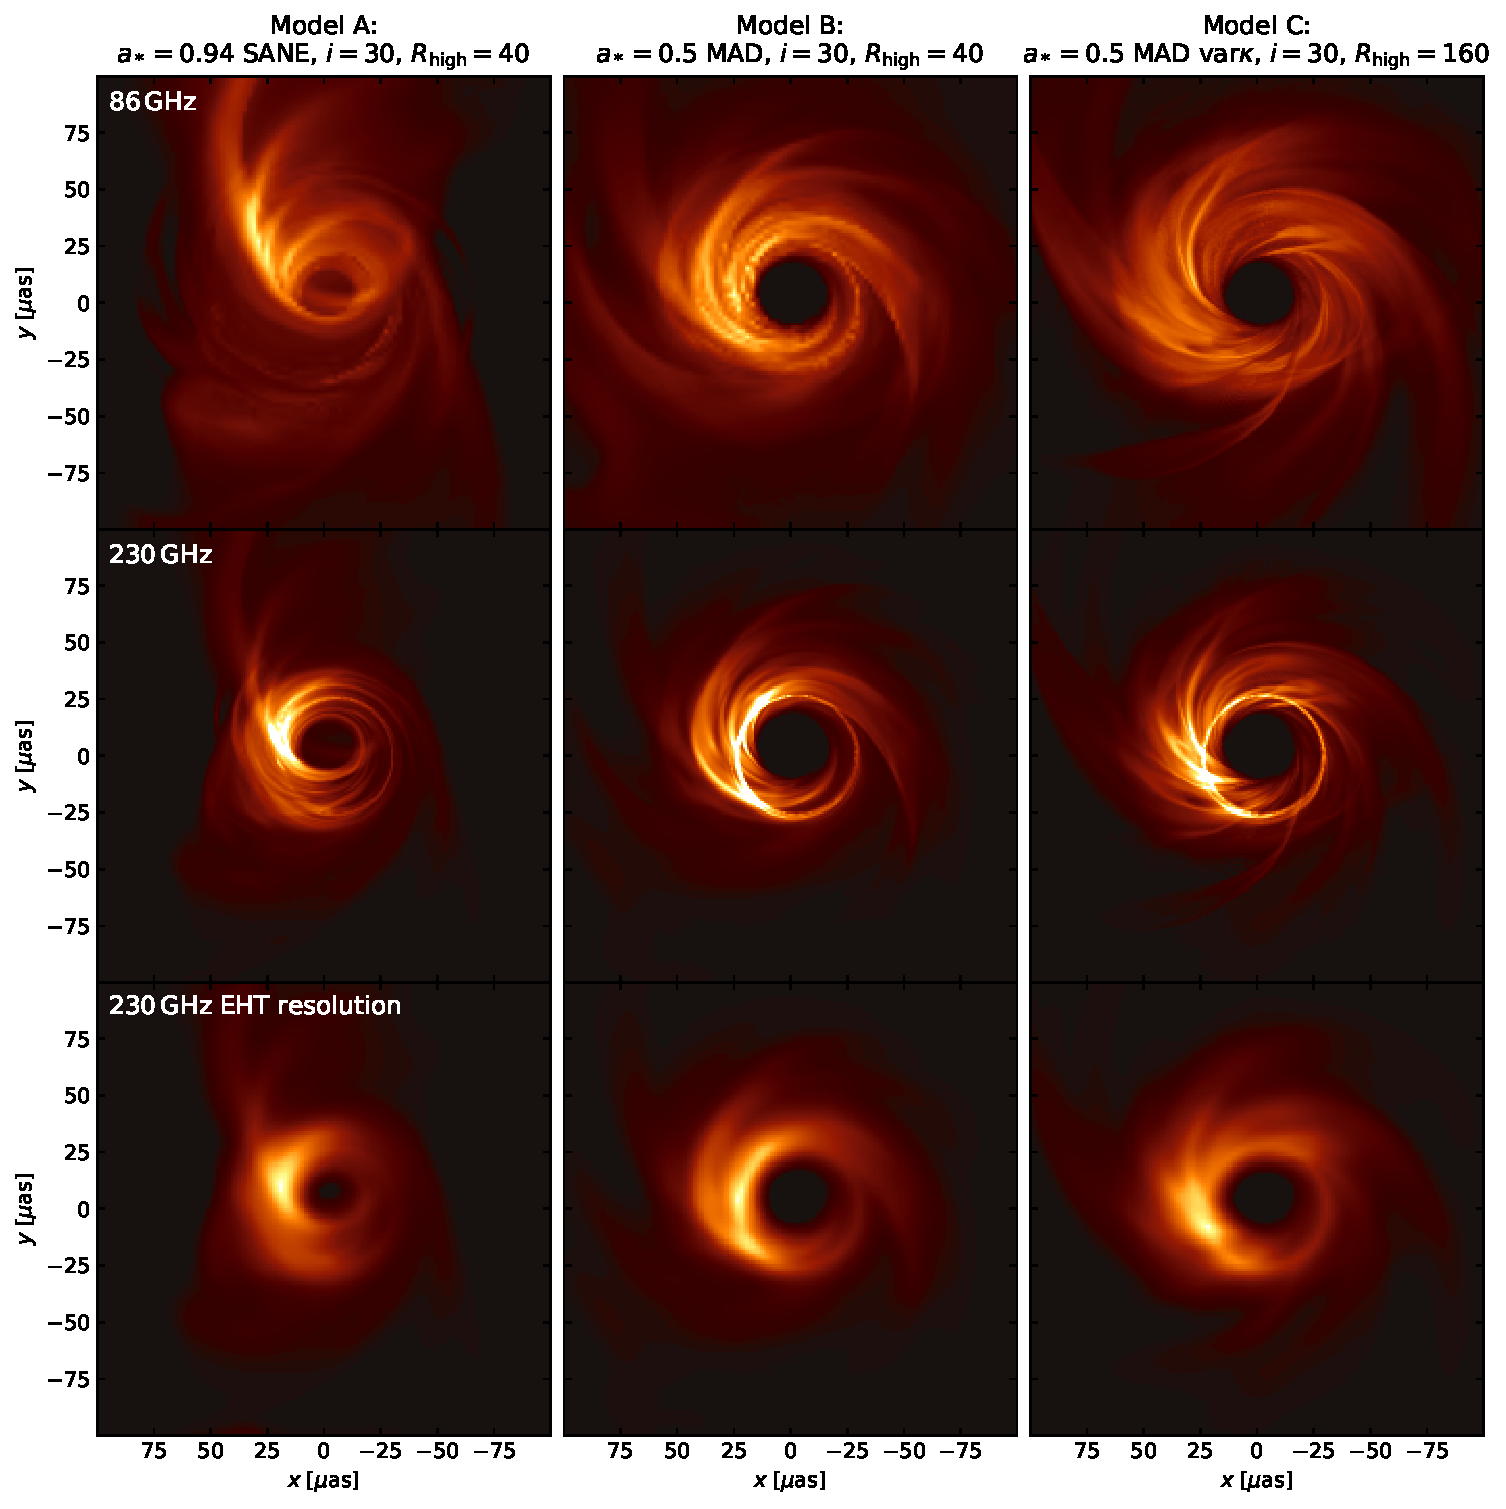
\includegraphics[width=\textwidth]{figures/bestbet_imgs.pdf}
  \caption{We show here the 86\GHz and 230\GHz ray traced images of
    the feature models.
    The different columns are Models~A, B, and C, respectively (see
    figure title or Table~\ref{tab:bestbets} for model description).
    The top row shows the simulated 86\GHz images, the middle row
    shows the simulated 230\GHz images, and the bottom row shows the
    simulated 230\GHz images filtered by a Butterworth filter at
    10$\,\mathrm{G}\lambda$, which approximate the resolution of the
    2017 EHT array.}
  \label{fig:bestbet_imgs}
\end{figure*}

\ckc{We don't have pizza plot for all the constraints now in the main
  text?}

We selected and applied 11 observational constraints in this section.
We now consider combining all constraints, excluding variability,
under the hypothesis that
\emph{i}) there is a missing physical ingredient in the models that
would lower variability, but
\emph{ii}) that missing ingredient would not vitiate the model
comparison process entirely.

The 6 EHT derived constraints are most constraining on the ring size
and width, roughly reduce the dimension of the parameter space by two,
and carving out a region of the parameter space that prefers prograde
models at low-to-intermediate inclinations
(Figure~\ref{fig:all_EHT_constraints}).

The 5 non-EHT constraints are most constraining on the strength of the
horizon magnetic field and the electron temperature, roughly reduce
the dimension of the parameter space by another two, and prefer high
ion-electron ratio MAD models (Figure~\ref{fig:non_eht_cuts}).

While there are also isolated pockets in the parameter space that pass
many constraints, however, even with an extensive study like this, it
is difficult to draw strong conclusion about these regions.

Among the tens of models that pass 10/11 constraints (see
Appendix~\ref{app:tables}), we feature three models in this section,
summarized in Table~\ref{tab:bestbets}.
These models are selected because they represent the different
magnetic field strength (both SANE and MAD) and eDFs (both thermal and
nonthermal), and represent clusters of passing models in the parameter
space.

In Figure~\ref{fig:bestbets}, we shows the visibility amplitudes and
SEDs of the the feature models and compare them with both EHT and
non-EHT data.
In both panels, symbols in black are from observations; blue is
Model~A ($\abh=0.94$ SANE, $\Rh=40$, $i=30$); orange is Model~B
($\abh=0.5$ MAD, $\Rh=40$, $i=30$); and green is Model~C ($\abh=0.5$
MAD variable $\kappa$, $\Rh=160$, $i=30$); see
Table~\ref{tab:bestbets}.

In the left panel, we show the visibility amplitudes as function of
$(u, v)$ distance similar to Figure~\ref{fig:passfail_va}.
For the observation, we plot 10\sec incoherent averaged data from the
HOPS pipeline on \aprilvii.
For the models, the solid curves are the VAs for only the position
angle $0\degree$ (parallel to the spin axis) for a particular
snapshot.
while the transparent bands show the 1 to 99 percentiles for all
position angles and all time.
This panel shows that the feature models agree well with the EHT VLBI
data.

In the right panel, we show the SEDs for the feature models and again
compare them with the observation constraints.
The solid lines are the mean SEDs, while the transparent bands show
the range across different snapshots.

In Figure~\ref{fig:bestbet_imgs}, we show the 86\GHz and 230\GHz ray
traced images of the feature models.
The different columns are Models~A, B, and C, respectively.
The top row shows the simulated 86\GHz images, the middle row shows
the simulated 230\GHz images, and the bottom row shows the simulated
230\GHz images filtered by a Butterworth filter at
10$\,\mathrm{G}\lambda$, which approximate the resolution of the 2017
EHT array \citep{2020arXiv200406210P}.

On one hand, although Model~A looks different than Model~B and C, they
pass all the constraints (excluding variability) we described in this
paper.
On the other hand, Model~B and C, even though one is thermal and the
other is nonthermal, look remarkable similar at 230\GHz.
The former point suggests that there is still ambiguity in the image
morphology, consistent with \citetalias{PaperIII, PaperIV}'s
conclusions.
The later point suggests that even for the same image morphology,
there are still degeneracy in the eDF, suggesting the importance of
new multiwavelength observations.
